\documentclass[]{article}

\usepackage{setspace}
\usepackage{lscape}
\usepackage{tikz}
\usepackage{float}
\def\checkmark{\tikz\fill[scale=0.4](0,.35) -- (.25,0) -- (1,.7) -- (.25,.15) -- cycle;} 
\usepackage{adjustbox,lipsum}
\usepackage{graphicx}
\usepackage{rotating}
\usepackage[section]{placeins}
\usepackage[left=1in, right=1in, top=1in]{geometry}
\renewcommand{\arraystretch}{.7}
\doublespacing
\renewcommand\thefigure{S\arabic{figure}}
\setcounter{figure}{0}    
\renewcommand\thetable{S\arabic{table}}    
\setcounter{table}{0}

\title{\vspace{-4em}Supplementary Materials for ``How `Rage Bait' and Outgroup Cues Strengthen Support for Violence and Anti-Muslim Policies''}

\begin{document}

\maketitle 
\tableofcontents
\newpage
\setcounter{page}{1}
\section{Sampling Procedures}

We recruited our respondents through Amazon Mechanical Turk in early December 2018. We advertised the Human Intelligence Task (HIT) as a study on media consumption behavior and compensated respondents 2.11 USD for taking our 15-minute survey, which corresponded to the hourly rate of the federal minimum wage in 2018. After consenting to the take survey, respondents were directed to an external website that hosted an embedded pre-treatment and post-treatment survey (hosted through Qualtrics) as well as the AP-styled news website and article. 

\subsection{Website Design and Randomization}

The interactive survey web app was custom coded using the Python Django web framework and deployed to the web using the Amazon Elastic Beanstalk service. It was designed to be responsive, working on any screen size or device. Click data, comments, and browser metadata were stored in a PostgreSQL database hosted on Amazon Relational Database Services (RDS).

In the web app view, we displayed the informed consent script. When respondents consented and continued to the next view, they were asked to provide their MTurk Worker ID to ensure that they did not fill out the survey twice. They were then asked to share their location to ensure that they were located within the United States. After these first two views, respondents were taken to the pre-treatment survey, followed by the article vignette.

We reverse-engineered the AP website article view for our vignette to maximize its credibility and, thereby, the external validity of our inferences. When the respondent loaded the article vignette, the web app randomly assigned them to one of eight possible treatment combinations which were dynamically displayed in a Django template view. After an interstitial loading page was displayed with a loading bar and a message reading, "Loading External Website...," the article vignette view loaded in an iframe below instructions for this portion of the survey.

Treatments were randomly assigned through the dynamic web-app which was hosted on Amazon Web Services (AWS). The web app assigned each respondent a randomly generated 4-character alphanumeric code. This code was used to match click, comment, and treatment assignment data with the respondent's Qualtrics survey responses. We manually checked survey codes for typographical errors to ensure proper matching.

The comment section was interactive, allowing users to like, report, and comment on the article. The web app tracked comments, likes, reports, and link clicks using AJAX to communicate between the web client and the PostgreSQL database. Each interaction was saved with the respondent's survey ID to facilitate matching these data with Qualtrics data.

\vspace{-1em}
\begin{figure}[!htbp]
  \centering
  \caption{Loading Interstitial for the Website}
  \vspace{1em}
  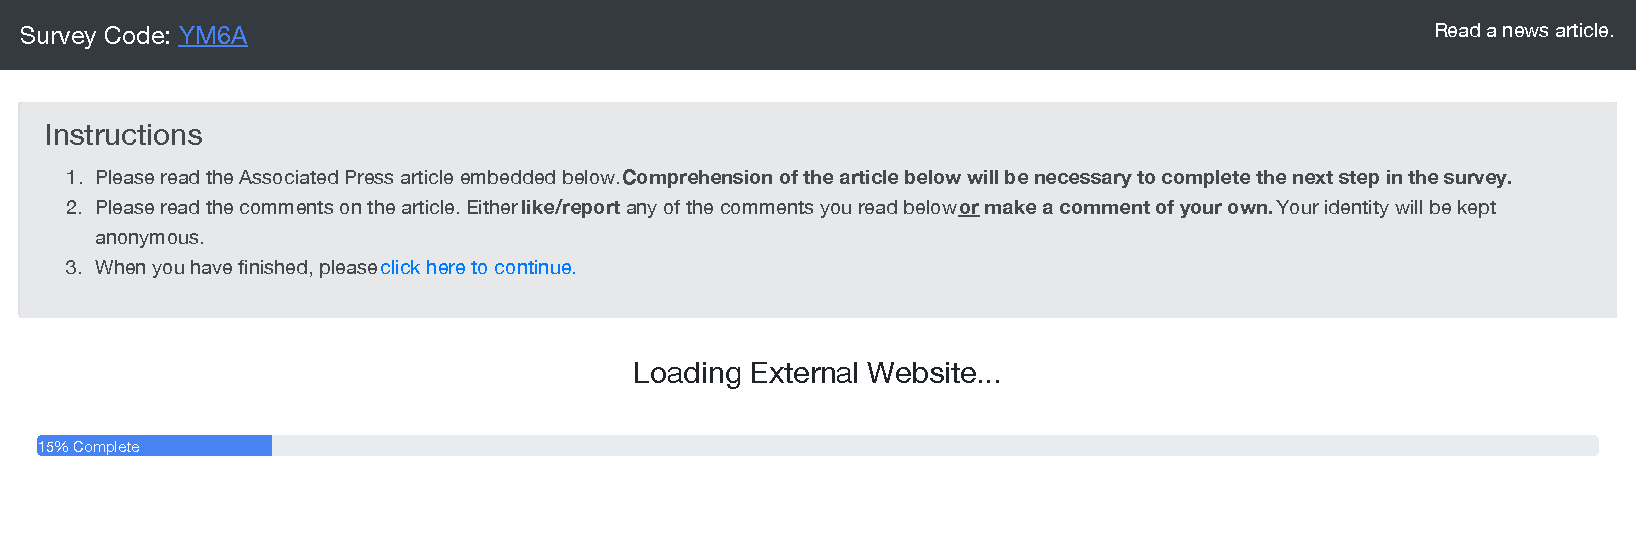
\includegraphics[width=.9\textwidth]{figures/loading_interstitial.pdf}\\
  \label{hom_uns}
\end{figure}

\subsection{Exclusion Criteria}

We drew an initial sample of 1879 respondents, of which we excluded 224 according to the following criteria.

\textit{Bots and Fraudulent Accounts.} Many accounts on the Amazon Mechanical Turk platform are fraudulent and needed to be screened out of our data. We anticipated this and used four methods to screen them out of our data. First, we required users to enter a survey completion code on the Amazon Mechanical Turk platform. This code was displayed to them after completion of the survey. They were also required to provide their MTurk ID within the survey to ensure that their response could be matched to their MTurk account. This limited each MTurk ID to one survey response. Second, because many fraudulent users simultaneously take surveys from multiple MTurk accounts, we collected data on the user's device (screen size, battery level, browser, etc.), location, and IP address to identify users who are completing the survey multiple times from the same machine. Third, to identify automated survey responses from bots, we read every open-ended response and excluded obvious machine-generated text or text scraped from the internet using reference words from the open-ended questions. 

\textit{Attention Check Failure.} We asked a very simple attention check question at the end of the survey. After reviewing failed attention checks, most were from accounts that appeared to be automated. Those who failed the attention check but did not appear to be bots were kept in the sample.

\textit{Duplicates.} Many subjects took the survey several times due to an error in our screening procedure that was fixed early on. For these subjects we dropped all but the first response from our sample using their MTurk ID, as described above.

\textit{Extreme Non-compliers.} Respondents who finished the survey in under 7 minutes were excluded, since it was not within reasonable expectations that they could have completed the survey within that amount of time.

\textit{Non-US Residents.} Since our relevant population was US residents, we required respondents to reside in the United States. However, because MTurk's screening criteria is not perfect, several respondents who were from outside the United States took the survey. We screened these respondents by using geolocation and IP address filters and identifying non-English open-ended responses.

\section{Survey Experiment Vignettes}

\subsection{Article Vignettes}

\begin{figure}[!htbp]
  \centering
  \caption{Vignette with Objective Content and Unspecified Perpetrator}
  \vspace{1em}
  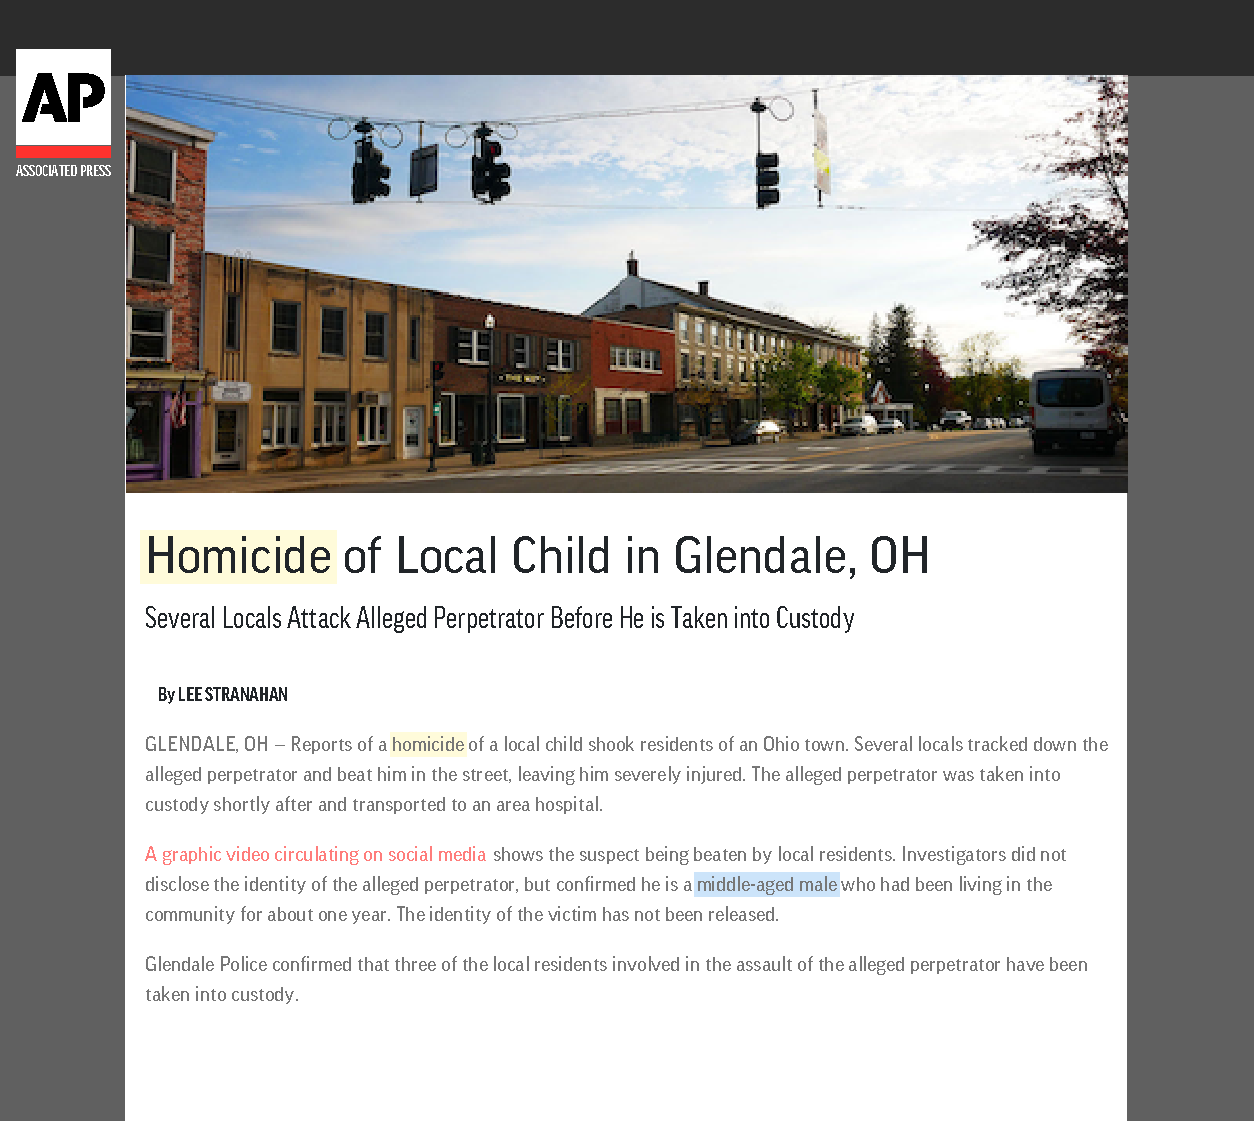
\includegraphics[width=.75\textwidth]{figures/hom_uns.pdf}\\
  \label{hom_uns}
\end{figure}

\begin{figure}
  \centering
  \caption{Vignette with Moral-Emotional Content and Muslim Refugee Perpetrator}
  \vspace{1em}
  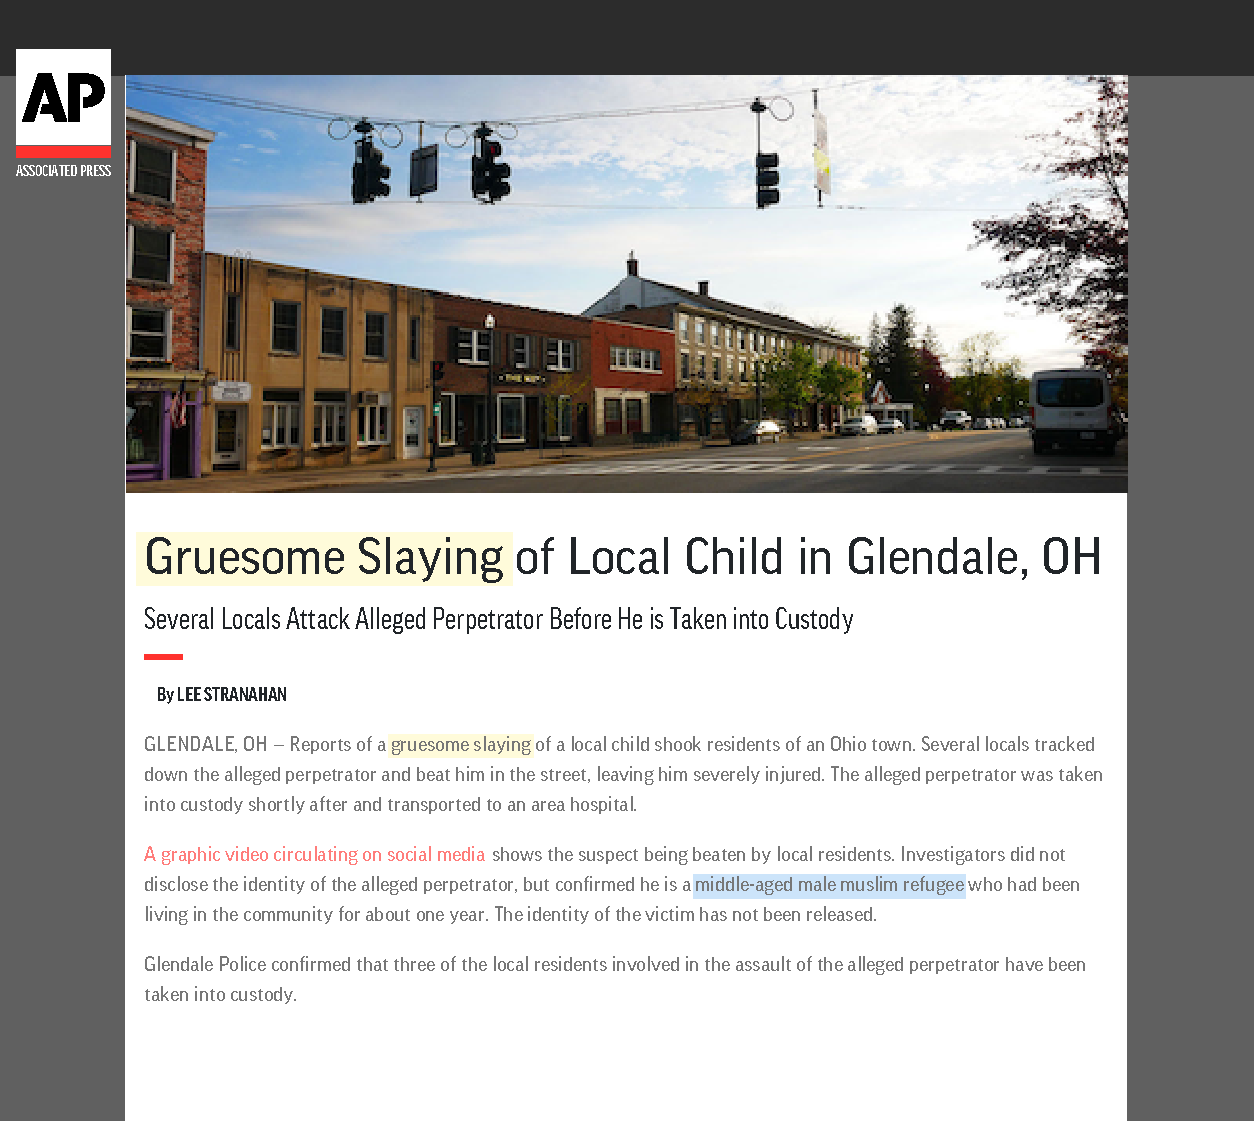
\includegraphics[width=.75\textwidth]{figures/hom_mus.pdf}\\
  \label{hom_mus}
\end{figure}

\begin{figure}
  \centering
  \caption{Comment List with Most Upvoted Violent Comment}
  \vspace{1em}
  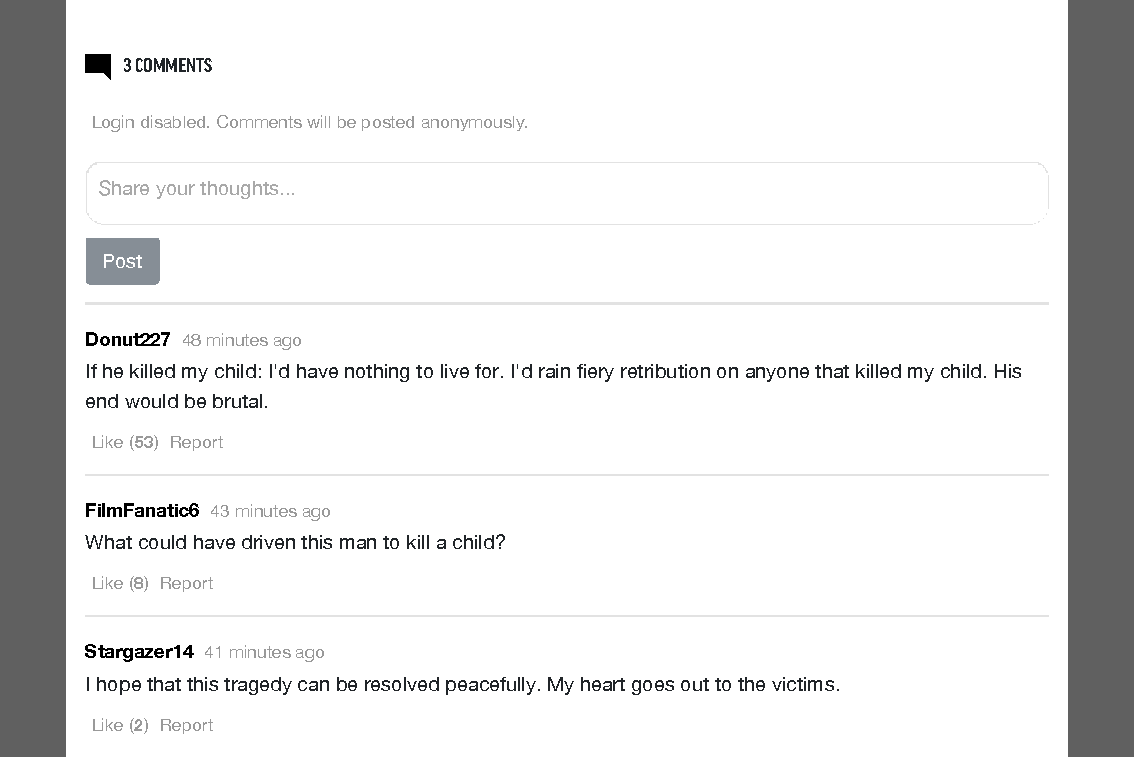
\includegraphics[width=.75\textwidth]{figures/comments.pdf}\\
  \label{com_vio}
\end{figure}

\begin{figure}
  \centering
  \caption{Comment List with Most Upvoted Conciliatory Comment }
  \vspace{1em}
  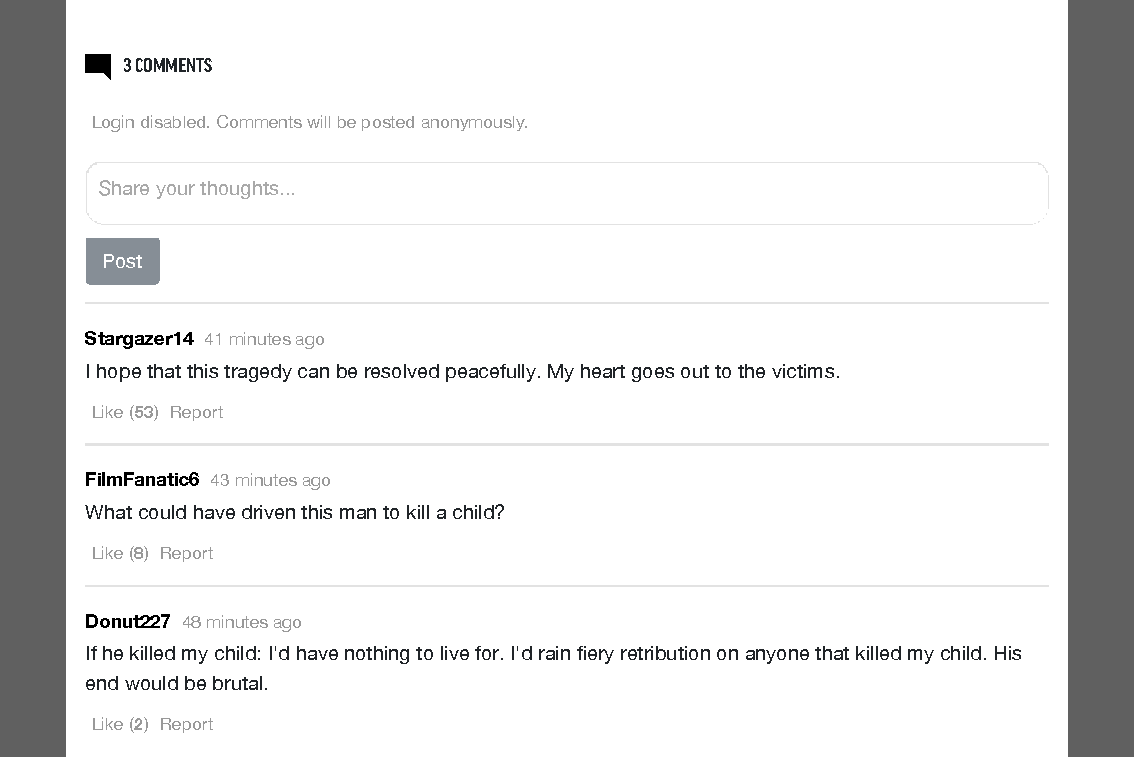
\includegraphics[width=.75\textwidth]{figures/comments_2.pdf}\\
  \label{com_neu}
\end{figure}

\newpage

\section{Measurement Validity Checks}

\begin{figure}[H]
  \centering
  \caption{Correlation of Measures of Support for Violence}
  \vspace{1em}
  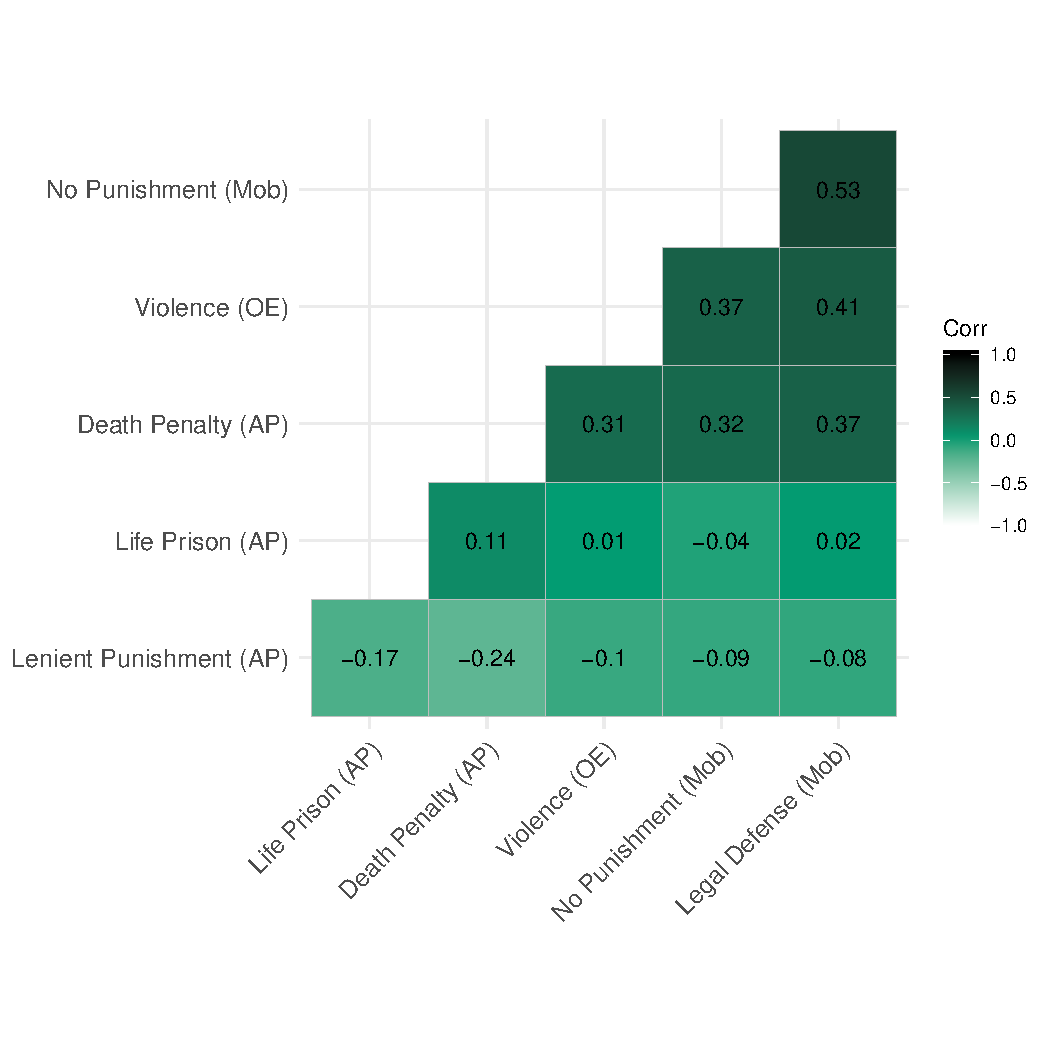
\includegraphics[width=.7\textwidth]{figures/corr_plot.pdf}\\
\end{figure}


\begin{table}[H] \centering 
  \caption{Willingness to Donate to Legal Defense Fund for Mob Attackers and Expressed Support for Extrajudicial Violence in Open-ended Responses} 
  \label{} 
\begin{tabular}{@{\extracolsep{5pt}}lc} 
\\[-1.8ex]\hline 
\hline \\[-1.8ex] 
 & \multicolumn{1}{c}{\textit{Dependent variable:}} \\ 
\cline{2-2} 
 & Extrajudicial \\ 
\hline \\[-1.8ex] 
 Legal Defense Fund & 0.118$^{***}$ \\ 
  & (0.005) \\ 
  & \\ 
\hline \\[-1.8ex] 
Observations & 1,602 \\ 
\hline 
\hline \\[-1.8ex] 
\textit{Note:}  & \multicolumn{1}{r}{$^{*}$p$<$0.1; $^{**}$p$<$0.05; $^{***}$p$<$0.01} \\ 
\end{tabular} 
\end{table} 


%\newpage

%\section{Descriptive Statistics}

%
\begin{table}[H] \centering 
  \caption{Descriptive Statistics for Survey Responses} 
  \label{} 
\begin{tabular}{@{\extracolsep{5pt}}lccccc} 
\\[-1.8ex]\hline 
\hline \\[-1.8ex] 
Statistic & \multicolumn{1}{c}{N} & \multicolumn{1}{c}{Mean} & \multicolumn{1}{c}{St. Dev.} & \multicolumn{1}{c}{Min} & \multicolumn{1}{c}{Max} \\ 
\hline \\[-1.8ex] 
age & 1,655 & 38.671 & 11.868 & 18 & 82 \\ 
education & 1,655 & 4.184 & 1.313 & 1 & 7 \\ 
auth\_log & 1,655 & 0.700 & 0.626 & 0.000 & 1.609 \\ 
ethno\_og & 1,655 & 33.624 & 18.564 & 0.000 & 95.933 \\ 
symb\_rac\_log & 1,655 & 1.231 & 0.373 & 0.693 & 1.792 \\ 
emo\_ang\_hom & 1,650 & 3.610 & 1.271 & 1.000 & 5.000 \\ 
emo\_sat\_hom & 1,650 & 1.176 & 0.613 & 1.000 & 5.000 \\ 
emo\_sad\_hom & 1,650 & 3.949 & 1.153 & 1.000 & 5.000 \\ 
emo\_dis\_hom & 1,650 & 3.853 & 1.203 & 1.000 & 5.000 \\ 
emo\_hap\_hom & 1,650 & 1.081 & 0.434 & 1.000 & 5.000 \\ 
emo\_fea\_hom & 1,650 & 2.178 & 1.270 & 1.000 & 5.000 \\ 
emo\_anx\_hom & 1,650 & 2.402 & 1.257 & 1.000 & 5.000 \\ 
pun\_nopu\_hom & 1,632 & $-$2.836 & 0.740 & $-$3.000 & 3.000 \\ 
pun\_comm\_hom & 1,632 & $-$1.947 & 1.846 & $-$3.000 & 3.000 \\ 
pun\_short\_pris\_hom & 1,632 & $-$2.423 & 1.253 & $-$3.000 & 3.000 \\ 
pun\_long\_pris\_hom & 1,632 & 1.965 & 1.693 & $-$3.000 & 3.000 \\ 
pun\_life\_pris\_hom & 1,632 & 2.350 & 1.285 & $-$3.000 & 3.000 \\ 
pun\_exe\_inje\_hom & 1,632 & 1.015 & 2.152 & $-$3.000 & 3.000 \\ 
pun\_exe\_fire\_hom & 1,632 & 0.105 & 2.353 & $-$3.000 & 3.000 \\ 
pun\_exe\_hang\_hom & 1,632 & 0.093 & 2.362 & $-$3.000 & 3.000 \\ 
pun\_exe\_publ\_hom & 1,632 & $-$0.241 & 2.389 & $-$3.000 & 3.000 \\ 
torture & 1,632 & $-$1.055 & 2.095 & $-$3.000 & 3.000 \\ 
detain & 1,632 & $-$0.749 & 2.188 & $-$3.000 & 3.000 \\ 
pun\_nopu\_mob & 1,618 & $-$0.787 & 2.238 & $-$3.000 & 3.000 \\ 
pun\_comm\_mob & 1,618 & 0.770 & 2.093 & $-$3.000 & 3.000 \\ 
legal\_def & 1,618 & $-$0.777 & 1.998 & $-$3.000 & 3.000 \\ 
punitive\_hom & 1,616 & 0.954 & 1.376 & $-$3.000 & 3.000 \\ 
punitive\_refugee & 1,616 & $-$0.295 & 1.889 & $-$3.000 & 3.000 \\ 
punitive\_mus\_imm & 1,615 & $-$0.268 & 1.734 & $-$3.000 & 3.000 \\ 
punitive\_mus\_mon & 1,615 & $-$0.159 & 1.725 & $-$3.000 & 3.000 \\ 
punitive\_mus\_reg & 1,615 & $-$0.865 & 2.058 & $-$3.000 & 3.000 \\ 
\hline \\[-1.8ex] 
\end{tabular} 
\end{table} 

%
\begin{table}[H] \centering 
  \caption{Descriptive Statistics for Behavioral Indicators} 
  \label{} 
\begin{tabular}{@{\extracolsep{5pt}}lccccc} 
\\[-1.8ex]\hline 
\hline \\[-1.8ex] 
Statistic & \multicolumn{1}{c}{N} & \multicolumn{1}{c}{Mean} & \multicolumn{1}{c}{St. Dev.} & \multicolumn{1}{c}{Min} & \multicolumn{1}{c}{Max} \\ 
\hline \\[-1.8ex] 
video\_link & 1,655 & 0.356 & 0.479 & 0 & 1 \\ 
com\_viol\_report & 1,655 & 0.355 & 0.479 & 0 & 1 \\ 
com\_info\_report & 1,655 & 0.293 & 0.455 & 0 & 1 \\ 
com\_pos\_report & 1,655 & 0.293 & 0.455 & 0 & 1 \\ 
com\_viol\_like & 1,655 & 0.538 & 0.499 & 0 & 1 \\ 
com\_info\_like & 1,655 & 0.589 & 0.492 & 0 & 1 \\ 
com\_pos\_like & 1,655 & 0.749 & 0.434 & 0 & 1 \\ 
commenter & 1,655 & 0.304 & 0.460 & 0 & 1 \\ 
violence\_com & 499 & 0.263 & 0.440 & 0.000 & 1.000 \\ 
lethal\_com & 499 & 0.056 & 0.230 & 0.000 & 1.000 \\ 
extrajudicial\_com & 499 & 0.212 & 0.409 & 0.000 & 1.000 \\ 
dehumanizing\_com & 499 & 0.010 & 0.100 & 0.000 & 1.000 \\ 
demonizing\_com & 499 & 0.026 & 0.159 & 0.000 & 1.000 \\ 
group\_com & 499 & 0.052 & 0.222 & 0.000 & 1.000 \\ 
ingroup\_com & 499 & 0.082 & 0.275 & 0.000 & 1.000 \\ 
anger\_com & 499 & 0.012 & 0.109 & 0.000 & 1.000 \\ 
disgust\_com & 499 & 0.028 & 0.165 & 0.000 & 1.000 \\ 
sadness\_com & 499 & 0.279 & 0.449 & 0.000 & 1.000 \\ 
fear\_com & 499 & 0.012 & 0.109 & 0.000 & 1.000 \\ 
anxiety\_com & 499 & 0.006 & 0.077 & 0.000 & 1.000 \\ 
\hline \\[-1.8ex] 
\end{tabular} 
\end{table} 

%
\begin{table}[H] \centering 
  \caption{Descriptive Statistics for Open-ended Responses} 
  \label{} 
\begin{tabular}{@{\extracolsep{5pt}}lccccc} 
\\[-1.8ex]\hline 
\hline \\[-1.8ex] 
Statistic & \multicolumn{1}{c}{N} & \multicolumn{1}{c}{Mean} & \multicolumn{1}{c}{St. Dev.} & \multicolumn{1}{c}{Min} & \multicolumn{1}{c}{Max} \\ 
\hline \\[-1.8ex] 
violence\_oe & 1,616 & 0.537 & 0.499 & 0.000 & 1.000 \\ 
lethal\_oe & 1,616 & 0.101 & 0.302 & 0.000 & 1.000 \\ 
extrajudicial\_oe & 1,616 & 0.377 & 0.485 & 0.000 & 1.000 \\ 
dehumanizing\_oe & 1,616 & 0.030 & 0.170 & 0.000 & 1.000 \\ 
demonizing\_oe & 1,616 & 0.116 & 0.320 & 0.000 & 1.000 \\ 
group\_oe & 1,616 & 0.097 & 0.296 & 0.000 & 1.000 \\ 
ingroup\_oe & 1,616 & 0.196 & 0.397 & 0.000 & 1.000 \\ 
anger\_oe & 1,616 & 0.121 & 0.327 & 0.000 & 1.000 \\ 
disgust\_oe & 1,616 & 0.248 & 0.432 & 0.000 & 1.000 \\ 
sadness\_oe & 1,616 & 0.594 & 0.491 & 0.000 & 1.000 \\ 
fear\_oe & 1,616 & 0.100 & 0.300 & 0.000 & 1.000 \\ 
anxiety\_oe & 1,616 & 0.025 & 0.157 & 0.000 & 1.000 \\ 
\hline \\[-1.8ex] 
\end{tabular} 
\end{table} 


%\newpage
%\vspace{-1em}

\section{Attitudes Towards Violence}\vspace{-1em}

\begin{figure}[!htbp]
  \centering
  \caption{Support for Judicial and Extrajudicial Punishment by Treatment Condition (Direct Measures)}
  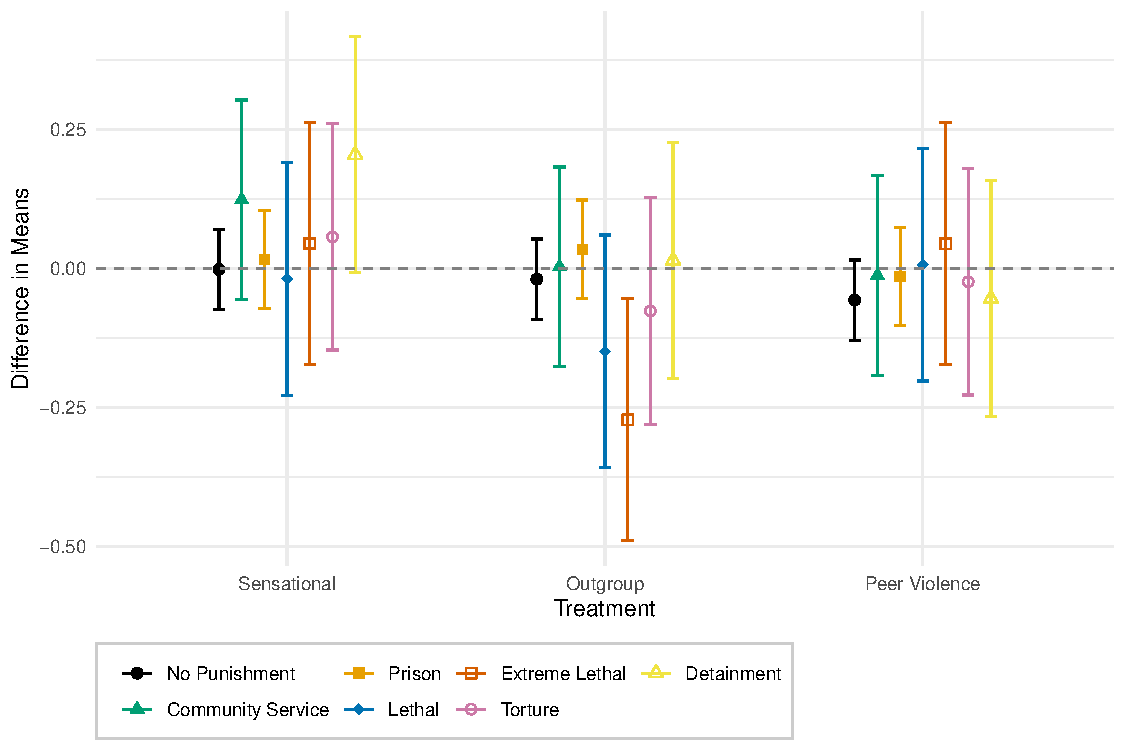
\includegraphics[width=\textwidth]{figures/ATE_punish_hom_outcomes.pdf}
\end{figure}
\subsection{Judicial Violence (Direct)}


\begin{table}[H] \centering 
  \caption{Attitudes Toward Judicial Punishment of the Alleged Perpetrator} 
  \label{} 
\resizebox{\textwidth}{!}{\begin{tabular}{@{\extracolsep{5pt}}lcccccccccccc} 
\\[-1.8ex]\hline 
\hline \\[-1.8ex] 
 & \multicolumn{12}{c}{\textit{Dependent variable:}} \\ 
\cline{2-13} 
 & Lenient & Lenient & Lenient & Prison & Prison & Prison & Lethal & Lethal & Lethal & Extreme Lethal & Extreme Lethal & Extreme Lethal \\ 
\\[-1.8ex] & (1) & (2) & (3) & (4) & (5) & (6) & (7) & (8) & (9) & (10) & (11) & (12)\\ 
\hline \\[-1.8ex] 
 Sensational & 0.060 & 0.058 & 0.060 & 0.015 & 0.006 & 0.007 & $-$0.019 & 0.019 & 0.016 & 0.044 & 0.099 & 0.092 \\ 
  & (0.053) & (0.053) & (0.053) & (0.045) & (0.045) & (0.045) & (0.107) & (0.099) & (0.098) & (0.111) & (0.102) & (0.102) \\ 
  & & & & & & & & & & & & \\ 
 Outgroup & $-$0.009 & 0.233 & 0.219 & 0.034 & 0.092 & 0.092 & $-$0.150 & $-$0.222 & $-$0.243 & $-$0.272$^{**}$ & $-$0.487 & $-$0.463 \\ 
  & (0.053) & (0.179) & (0.177) & (0.045) & (0.161) & (0.160) & (0.107) & (0.378) & (0.372) & (0.111) & (0.370) & (0.363) \\ 
  & & & & & & & & & & & & \\ 
 Peer Violence & $-$0.035 & $-$0.039 & $-$0.039 & $-$0.015 & $-$0.013 & $-$0.014 & 0.006 & 0.019 & 0.020 & 0.044 & 0.044 & 0.044 \\ 
  & (0.053) & (0.053) & (0.053) & (0.045) & (0.045) & (0.045) & (0.107) & (0.098) & (0.098) & (0.111) & (0.102) & (0.101) \\ 
  & & & & & & & & & & & & \\ 
 Auth. (Log) &  & $-$0.043 & $-$0.036 &  & $-$0.076 & $-$0.077 &  & 0.513$^{***}$ & 0.505$^{***}$ &  & 0.466$^{***}$ & 0.452$^{***}$ \\ 
  &  & (0.063) & (0.063) &  & (0.053) & (0.053) &  & (0.122) & (0.122) &  & (0.127) & (0.126) \\ 
  & & & & & & & & & & & & \\ 
 Ethno. &  & 0.003 &  &  & $-$0.003 &  &  & 0.007 &  &  & 0.013$^{***}$ &  \\ 
  &  & (0.003) &  &  & (0.002) &  &  & (0.004) &  &  & (0.004) &  \\ 
  & & & & & & & & & & & & \\ 
 Anti-Muslim Sentiment &  &  & 0.0002 &  &  & $-$0.002 &  &  & 0.008$^{**}$ &  &  & 0.015$^{***}$ \\ 
  &  &  & (0.002) &  &  & (0.002) &  &  & (0.003) &  &  & (0.003) \\ 
  & & & & & & & & & & & & \\ 
 Symb. Racism (Log) &  & $-$0.045 & $-$0.004 &  & $-$0.117 & $-$0.123 &  & 1.053$^{***}$ & 1.012$^{***}$ &  & 1.143$^{***}$ & 1.075$^{***}$ \\ 
  &  & (0.119) & (0.117) &  & (0.094) & (0.095) &  & (0.218) & (0.218) &  & (0.228) & (0.226) \\ 
  & & & & & & & & & & & & \\ 
 South &  & 0.088 & 0.084 &  & $-$0.017 & $-$0.014 &  & 0.110 & 0.105 &  & 0.220$^{**}$ & 0.199$^{*}$ \\ 
  &  & (0.056) & (0.056) &  & (0.046) & (0.046) &  & (0.102) & (0.102) &  & (0.107) & (0.106) \\ 
  & & & & & & & & & & & & \\ 
 Republican &  & $-$0.192$^{***}$ & $-$0.196$^{***}$ &  & $-$0.077 & $-$0.077 &  & 0.675$^{***}$ & 0.664$^{***}$ &  & 0.577$^{***}$ & 0.555$^{***}$ \\ 
  &  & (0.067) & (0.067) &  & (0.059) & (0.059) &  & (0.111) & (0.111) &  & (0.131) & (0.130) \\ 
  & & & & & & & & & & & & \\ 
 Outgroup x Auth. (Log) &  & $-$0.003 & $-$0.014 &  & 0.125 & 0.125 &  & 0.025 & 0.027 &  & $-$0.079 & $-$0.086 \\ 
  &  & (0.086) & (0.087) &  & (0.077) & (0.077) &  & (0.171) & (0.171) &  & (0.177) & (0.177) \\ 
  & & & & & & & & & & & & \\ 
 Outgroup x Ethno &  & 0.002 &  &  & 0.001 &  &  & $-$0.006 &  &  & 0.003 &  \\ 
  &  & (0.003) &  &  & (0.003) &  &  & (0.006) &  &  & (0.006) &  \\ 
  & & & & & & & & & & & & \\ 
 Outgroup x Anti-Muslim Sentiment &  &  & 0.004 &  &  & 0.001 &  &  & $-$0.004 &  &  & 0.001 \\ 
  &  &  & (0.003) &  &  & (0.002) &  &  & (0.005) &  &  & (0.005) \\ 
  & & & & & & & & & & & & \\ 
 Outgroup x Symb. Racism (Log) &  & $-$0.238 & $-$0.279$^{*}$ &  & $-$0.147 & $-$0.156 &  & 0.175 & 0.161 &  & 0.133 & 0.145 \\ 
  &  & (0.153) & (0.153) &  & (0.140) & (0.140) &  & (0.302) & (0.302) &  & (0.315) & (0.313) \\ 
  & & & & & & & & & & & & \\ 
\hline \\[-1.8ex] 
Observations & 1,629 &  &  & 1,629 &  &  & 1,629 &  &  & 1,629 &  &  \\ 
\hline 
\hline \\[-1.8ex] 
\textit{Note:}  & \multicolumn{12}{r}{$^{*}$p$<$0.1; $^{**}$p$<$0.05; $^{***}$p$<$0.01} \\ 
\end{tabular}} 
\end{table} 


\subsection{Extrajudicial Violence (Direct)}


\begin{table}[H] \centering 
  \caption{Direct Questions About Extrajudicial Punishment of the Alleged Perpetrator} 
  \label{} 
\begin{tabular}{@{\extracolsep{5pt}}lcccccc} 
\\[-1.8ex]\hline 
\hline \\[-1.8ex] 
 & \multicolumn{6}{c}{\textit{Dependent variable:}} \\ 
\cline{2-7} 
 & Torture & Torture & Torture & Detainment & Detainment & Detainment \\ 
\\[-1.8ex] & (1) & (2) & (3) & (4) & (5) & (6)\\ 
\hline \\[-1.8ex] 
 Sensational & 0.057 & 0.083 & 0.081 & 0.204$^{*}$ & 0.224$^{**}$ & 0.220$^{**}$ \\ 
  & (0.104) & (0.097) & (0.097) & (0.108) & (0.104) & (0.104) \\ 
  & & & & & & \\ 
 Outgroup & $-$0.077 & 0.031 & 0.006 & 0.014 & $-$0.314 & $-$0.279 \\ 
  & (0.104) & (0.331) & (0.327) & (0.108) & (0.357) & (0.352) \\ 
  & & & & & & \\ 
 Peer Violence & $-$0.024 & $-$0.018 & $-$0.017 & $-$0.055 & $-$0.041 & $-$0.042 \\ 
  & (0.104) & (0.097) & (0.096) & (0.108) & (0.104) & (0.104) \\ 
  & & & & & & \\ 
 Auth. (Log) &  & 0.659$^{***}$ & 0.656$^{***}$ &  & 0.680$^{***}$ & 0.670$^{***}$ \\ 
  &  & (0.121) & (0.121) &  & (0.127) & (0.127) \\ 
  & & & & & & \\ 
 Ethno. &  & 0.016$^{***}$ &  &  & 0.006 &  \\ 
  &  & (0.004) &  &  & (0.004) &  \\ 
  & & & & & & \\ 
 Anti-Muslim Sentiment &  &  & 0.014$^{***}$ &  &  & 0.008$^{**}$ \\ 
  &  &  & (0.003) &  &  & (0.004) \\ 
  & & & & & & \\ 
 Symb. Racism (Log) &  & 0.833$^{***}$ & 0.839$^{***}$ &  & 0.381 & 0.327 \\ 
  &  & (0.225) & (0.224) &  & (0.232) & (0.231) \\ 
  & & & & & & \\ 
 South &  & 0.268$^{***}$ & 0.246$^{**}$ &  & 0.230$^{**}$ & 0.218$^{**}$ \\ 
  &  & (0.101) & (0.100) &  & (0.108) & (0.108) \\ 
  & & & & & & \\ 
 Republican &  & 0.100 & 0.075 &  & 0.241$^{*}$ & 0.229$^{*}$ \\ 
  &  & (0.130) & (0.130) &  & (0.137) & (0.137) \\ 
  & & & & & & \\ 
 Outgroup x Auth. (Log) &  & 0.127 & 0.107 &  & 0.043 & 0.040 \\ 
  &  & (0.170) & (0.170) &  & (0.180) & (0.179) \\ 
  & & & & & & \\ 
 Outgroup x Ethno &  & $-$0.0001 &  &  & 0.005 &  \\ 
  &  & (0.005) &  &  & (0.006) &  \\ 
  & & & & & & \\ 
 Outgroup x Anti-Muslim Sentiment &  &  & 0.003 &  &  & 0.003 \\ 
  &  &  & (0.005) &  &  & (0.005) \\ 
  & & & & & & \\ 
 Outgroup x Symb. Racism (Log) &  & $-$0.169 & $-$0.234 &  & 0.093 & 0.118 \\ 
  &  & (0.307) & (0.308) &  & (0.321) & (0.322) \\ 
  & & & & & & \\ 
\hline \\[-1.8ex] 
Observations & 1,629 &  &  & 1,629 &  &  \\ 
\hline 
\hline \\[-1.8ex] 
\textit{Note:}  & \multicolumn{6}{r}{$^{*}$p$<$0.1; $^{**}$p$<$0.05; $^{***}$p$<$0.01} \\ 
\end{tabular} 
\end{table} 


\subsection{Extrajudicial Violence (Indirect)}


\begin{table}[H] \centering 
  \caption{Indirect Questions About Extrajudicial Punishment of the Alleged Perpetrator} 
  \label{} 
\resizebox{\textwidth}{!}{\begin{tabular}{@{\extracolsep{5pt}}lccccccccc} 
\\[-1.8ex]\hline 
\hline \\[-1.8ex] 
 & \multicolumn{9}{c}{\textit{Dependent variable:}} \\ 
\cline{2-10} 
 & No Punish. & No Punish. & No Punish. & Comm. Service & Comm. Service & Comm. Service & Leg. Defense & Leg. Defense & Leg. Defense \\ 
\\[-1.8ex] & (1) & (2) & (3) & (4) & (5) & (6) & (7) & (8) & (9)\\ 
\hline \\[-1.8ex] 
 Sensational & 0.164 & 0.203$^{*}$ & 0.197$^{*}$ & 0.052 & 0.054 & 0.055 & 0.217$^{**}$ & 0.250$^{***}$ & 0.247$^{***}$ \\ 
  & (0.111) & (0.108) & (0.108) & (0.104) & (0.104) & (0.104) & (0.099) & (0.096) & (0.096) \\ 
  & & & & & & & & & \\ 
 Outgroup & $-$0.285$^{**}$ & $-$1.005$^{***}$ & $-$0.975$^{***}$ & $-$0.205$^{**}$ & 0.067 & 0.054 & $-$0.083 & $-$0.842$^{**}$ & $-$0.843$^{**}$ \\ 
  & (0.111) & (0.378) & (0.373) & (0.104) & (0.379) & (0.374) & (0.099) & (0.337) & (0.331) \\ 
  & & & & & & & & & \\ 
 Peer Violence & 0.152 & 0.145 & 0.146 & 0.168 & 0.166 & 0.166 & 0.024 & 0.027 & 0.024 \\ 
  & (0.111) & (0.107) & (0.107) & (0.104) & (0.104) & (0.104) & (0.099) & (0.095) & (0.095) \\ 
  & & & & & & & & & \\ 
 Auth. (Log) &  & 0.314$^{**}$ & 0.303$^{**}$ &  & $-$0.188 & $-$0.187 &  & 0.434$^{***}$ & 0.425$^{***}$ \\ 
  &  & (0.137) & (0.136) &  & (0.134) & (0.133) &  & (0.126) & (0.125) \\ 
  & & & & & & & & & \\ 
 Ethno. &  & 0.011$^{**}$ &  &  & $-$0.003 &  &  & 0.005 &  \\ 
  &  & (0.004) &  &  & (0.004) &  &  & (0.004) &  \\ 
  & & & & & & & & & \\ 
 Anti-Muslim Sentiment &  &  & 0.011$^{***}$ &  &  & $-$0.003 &  &  & 0.007$^{**}$ \\ 
  &  &  & (0.004) &  &  & (0.004) &  &  & (0.003) \\ 
  & & & & & & & & & \\ 
 Symb. Racism (Log) &  & 0.349 & 0.304 &  & 0.034 & 0.035 &  & 0.280 & 0.230 \\ 
  &  & (0.247) & (0.248) &  & (0.239) & (0.241) &  & (0.221) & (0.221) \\ 
  & & & & & & & & & \\ 
 South &  & 0.204$^{*}$ & 0.186$^{*}$ &  & $-$0.040 & $-$0.034 &  & 0.234$^{**}$ & 0.224$^{**}$ \\ 
  &  & (0.112) & (0.112) &  & (0.109) & (0.109) &  & (0.099) & (0.099) \\ 
  & & & & & & & & & \\ 
 Republican &  & 0.472$^{***}$ & 0.459$^{***}$ &  & 0.224$^{*}$ & 0.228$^{*}$ &  & 0.372$^{***}$ & 0.355$^{***}$ \\ 
  &  & (0.142) & (0.142) &  & (0.132) & (0.132) &  & (0.123) & (0.123) \\ 
  & & & & & & & & & \\ 
 Outgroup x Auth. (Log) &  & $-$0.079 & $-$0.084 &  & $-$0.253 & $-$0.249 &  & 0.042 & 0.032 \\ 
  &  & (0.188) & (0.188) &  & (0.185) & (0.185) &  & (0.169) & (0.168) \\ 
  & & & & & & & & & \\ 
 Outgroup x Ethno &  & 0.003 &  &  & $-$0.003 &  &  & 0.003 &  \\ 
  &  & (0.006) &  &  & (0.006) &  &  & (0.006) &  \\ 
  & & & & & & & & & \\ 
 Outgroup x Anti-Muslim Sentiment &  &  & 0.001 &  &  & $-$0.002 &  &  & 0.004 \\ 
  &  &  & (0.005) &  &  & (0.005) &  &  & (0.005) \\ 
  & & & & & & & & & \\ 
 Outgroup x Symb. Racism (Log) &  & 0.535 & 0.569$^{*}$ &  & $-$0.003 & $-$0.009 &  & 0.495$^{*}$ & 0.458 \\ 
  &  & (0.339) & (0.339) &  & (0.335) & (0.335) &  & (0.301) & (0.302) \\ 
  & & & & & & & & & \\ 
\hline \\[-1.8ex] 
Observations & 1,615 &  &  & 1,615 &  &  & 1,615 &  &  \\ 
\hline 
\hline \\[-1.8ex] 
\textit{Note:}  & \multicolumn{9}{r}{$^{*}$p$<$0.1; $^{**}$p$<$0.05; $^{***}$p$<$0.01} \\ 
\end{tabular}} 
\end{table} 


{\setstretch{1.25}
\section{Attitudes Towards Outgroups}\vspace{-1em}


\begin{table}[H] \centering 
  \caption{OLS Models for Attitudes Toward Outgroups} 
  \label{} 
\resizebox{\textwidth}{!}{\begin{tabular}{@{\extracolsep{5pt}}lcccccccccccc} 
\\[-1.8ex]\hline 
\hline \\[-1.8ex] 
 & \multicolumn{12}{c}{\textit{Dependent variable:}} \\ 
\cline{2-13} 
 & Refugees & Refugees & Refugees & Muslim Immigration & Muslim Immigration & Muslim Immigration & Monitoring & Monitoring & Monitoring & Registry & Registry & Registry \\ 
\\[-1.8ex] & (1) & (2) & (3) & (4) & (5) & (6) & (7) & (8) & (9) & (10) & (11) & (12)\\ 
\hline \\[-1.8ex] 
 Sensational & 0.173$^{*}$ & 0.103 & 0.108 & 0.066 & 0.004 & 0.017 & $-$0.077 & $-$0.032 & $-$0.042 & $-$0.008 & 0.035 & 0.024 \\ 
  & (0.094) & (0.069) & (0.069) & (0.086) & (0.067) & (0.064) & (0.086) & (0.073) & (0.072) & (0.103) & (0.084) & (0.082) \\ 
  & & & & & & & & & & & & \\ 
 Outgroup & $-$0.148 & $-$0.444$^{*}$ & $-$0.441$^{*}$ & $-$0.200$^{**}$ & $-$0.577$^{**}$ & $-$0.616$^{***}$ & 0.181$^{**}$ & 0.065 & 0.102 & 0.193$^{*}$ & 0.328 & 0.332 \\ 
  & (0.094) & (0.238) & (0.235) & (0.086) & (0.229) & (0.219) & (0.086) & (0.257) & (0.251) & (0.103) & (0.269) & (0.259) \\ 
  & & & & & & & & & & & & \\ 
 Peer Violence & $-$0.005 & 0.0003 & $-$0.001 & 0.009 & 0.021 & 0.023 & 0.090 & 0.084 & 0.084 & 0.091 & 0.098 & 0.097 \\ 
  & (0.094) & (0.069) & (0.068) & (0.086) & (0.066) & (0.064) & (0.086) & (0.072) & (0.071) & (0.103) & (0.083) & (0.081) \\ 
  & & & & & & & & & & & & \\ 
 Auth. (Log) &  & $-$0.408$^{***}$ & $-$0.402$^{***}$ &  & $-$0.377$^{***}$ & $-$0.350$^{***}$ &  & 0.472$^{***}$ & 0.452$^{***}$ &  & 0.864$^{***}$ & 0.841$^{***}$ \\ 
  &  & (0.087) & (0.087) &  & (0.082) & (0.078) &  & (0.090) & (0.088) &  & (0.107) & (0.105) \\ 
  & & & & & & & & & & & & \\ 
 Ethno. &  & $-$0.016$^{***}$ &  &  & $-$0.019$^{***}$ &  &  & 0.016$^{***}$ &  &  & 0.020$^{***}$ &  \\ 
  &  & (0.003) &  &  & (0.003) &  &  & (0.003) &  &  & (0.004) &  \\ 
  & & & & & & & & & & & & \\ 
 Anti-Muslim Sentiment &  &  & $-$0.014$^{***}$ &  &  & $-$0.022$^{***}$ &  &  & 0.018$^{***}$ &  &  & 0.022$^{***}$ \\ 
  &  &  & (0.002) &  &  & (0.002) &  &  & (0.003) &  &  & (0.003) \\ 
  & & & & & & & & & & & & \\ 
 Symb. Racism (Log) &  & $-$2.051$^{***}$ & $-$2.044$^{***}$ &  & $-$1.791$^{***}$ & $-$1.661$^{***}$ &  & 1.289$^{***}$ & 1.205$^{***}$ &  & 1.371$^{***}$ & 1.271$^{***}$ \\ 
  &  & (0.169) & (0.169) &  & (0.159) & (0.153) &  & (0.173) & (0.169) &  & (0.193) & (0.190) \\ 
  & & & & & & & & & & & & \\ 
 South &  & $-$0.135$^{*}$ & $-$0.113 &  & $-$0.155$^{**}$ & $-$0.125$^{*}$ &  & 0.122 & 0.097 &  & 0.292$^{***}$ & 0.264$^{***}$ \\ 
  &  & (0.072) & (0.071) &  & (0.069) & (0.066) &  & (0.076) & (0.075) &  & (0.089) & (0.087) \\ 
  & & & & & & & & & & & & \\ 
 Republican &  & $-$1.089$^{***}$ & $-$1.068$^{***}$ &  & $-$0.792$^{***}$ & $-$0.758$^{***}$ &  & 0.432$^{***}$ & 0.409$^{***}$ &  & 0.529$^{***}$ & 0.494$^{***}$ \\ 
  &  & (0.088) & (0.087) &  & (0.085) & (0.081) &  & (0.094) & (0.093) &  & (0.116) & (0.114) \\ 
  & & & & & & & & & & & & \\ 
 Outgroup x Auth. (Log) &  & $-$0.011 & 0.004 &  & 0.063 & 0.070 &  & 0.161 & 0.157 &  & 0.250$^{*}$ & 0.242 \\ 
  &  & (0.123) & (0.123) &  & (0.114) & (0.108) &  & (0.126) & (0.124) &  & (0.151) & (0.149) \\ 
  & & & & & & & & & & & & \\ 
 Outgroup x Ethno &  & $-$0.001 &  &  & $-$0.004 &  &  & 0.002 &  &  & $-$0.001 &  \\ 
  &  & (0.004) &  &  & (0.004) &  &  & (0.005) &  &  & (0.005) &  \\ 
  & & & & & & & & & & & & \\ 
 Outgroup x Anti-Muslim Sentiment &  &  & $-$0.002 &  &  & $-$0.002 &  &  & $-$0.001 &  &  & $-$0.001 \\ 
  &  &  & (0.003) &  &  & (0.003) &  &  & (0.004) &  &  & (0.004) \\ 
  & & & & & & & & & & & & \\ 
 Outgroup x Symb. Racism (Log) &  & 0.314 & 0.338 &  & 0.408$^{*}$ & 0.385$^{*}$ &  & $-$0.081 & $-$0.038 &  & $-$0.249 & $-$0.260 \\ 
  &  & (0.226) & (0.227) &  & (0.212) & (0.206) &  & (0.238) & (0.233) &  & (0.271) & (0.269) \\ 
  & & & & & & & & & & & & \\ 
\hline \\[-1.8ex] 
Observations & 1,613 &  &  & 1,612 &  &  & 1,612 &  &  & 1,612 &  &  \\ 
\hline 
\hline \\[-1.8ex] 
\textit{Note:}  & \multicolumn{12}{r}{$^{*}$p$<$0.1; $^{**}$p$<$0.05; $^{***}$p$<$0.01} \\ 
\end{tabular}} 
\end{table} 
\vspace{-1.5em}

\section{Behavioral Indicators}\vspace{-1em}


\begin{table}[H] \centering 
  \caption{OLS Models for Behavioral Indicators} 
  \label{} 
\resizebox{\textwidth}{!}{\begin{tabular}{@{\extracolsep{5pt}}lcccccccccccc} 
\\[-1.8ex]\hline 
\hline \\[-1.8ex] 
 & \multicolumn{12}{c}{\textit{Dependent variable:}} \\ 
\cline{2-13} 
 & Liked Viol. & Liked Viol. & Liked Viol. & Liked Non-viol. & Liked Non-viol. & Liked Non-viol. & Reported Viol. & Reported Viol. & Reported Viol. & Wrote Comment & Wrote Comment & Wrote Comment \\ 
\\[-1.8ex] & (1) & (2) & (3) & (4) & (5) & (6) & (7) & (8) & (9) & (10) & (11) & (12)\\ 
\hline \\[-1.8ex] 
 Sensational & 0.004 & 0.011 & 0.011 & $-$0.025 & $-$0.028 & $-$0.027 & $-$0.018 & $-$0.016 & $-$0.015 & 0.045$^{**}$ & 0.050$^{**}$ & 0.050$^{**}$ \\ 
  & (0.025) & (0.024) & (0.024) & (0.021) & (0.021) & (0.021) & (0.024) & (0.024) & (0.024) & (0.023) & (0.023) & (0.023) \\ 
  & & & & & & & & & & & & \\ 
 Outgroup & $-$0.014 & $-$0.044 & $-$0.051 & $-$0.013 & 0.054 & 0.044 & 0.034 & 0.068 & 0.057 & $-$0.006 & $-$0.085 & $-$0.080 \\ 
  & (0.025) & (0.084) & (0.083) & (0.021) & (0.072) & (0.071) & (0.024) & (0.082) & (0.081) & (0.023) & (0.080) & (0.079) \\ 
  & & & & & & & & & & & & \\ 
 Peer Violence & 0.049$^{**}$ & 0.050$^{**}$ & 0.050$^{**}$ & $-$0.096$^{***}$ & $-$0.095$^{***}$ & $-$0.096$^{***}$ & $-$0.034 & $-$0.035 & $-$0.035 & 0.027 & 0.026 & 0.026 \\ 
  & (0.025) & (0.024) & (0.024) & (0.021) & (0.021) & (0.021) & (0.024) & (0.024) & (0.024) & (0.023) & (0.023) & (0.023) \\ 
  & & & & & & & & & & & & \\ 
 Auth. (Log) &  & 0.042 & 0.042 &  & $-$0.015 & $-$0.013 &  & $-$0.022 & $-$0.020 &  & $-$0.002 & $-$0.002 \\ 
  &  & (0.029) & (0.029) &  & (0.025) & (0.025) &  & (0.029) & (0.028) &  & (0.028) & (0.028) \\ 
  & & & & & & & & & & & & \\ 
 Ethno. &  & $-$0.00002 &  &  & $-$0.002$^{**}$ &  &  & $-$0.001 &  &  & $-$0.001 &  \\ 
  &  & (0.001) &  &  & (0.001) &  &  & (0.001) &  &  & (0.001) &  \\ 
  & & & & & & & & & & & & \\ 
 Anti-Muslim Sentiment &  &  & 0.0001 &  &  & $-$0.002$^{***}$ &  &  & $-$0.001 &  &  & $-$0.001 \\ 
  &  &  & (0.001) &  &  & (0.001) &  &  & (0.001) &  &  & (0.001) \\ 
  & & & & & & & & & & & & \\ 
 Symb. Racism (Log) &  & 0.213$^{***}$ & 0.212$^{***}$ &  & $-$0.012 & 0.001 &  & 0.100$^{*}$ & 0.115$^{**}$ &  & 0.059 & 0.057 \\ 
  &  & (0.051) & (0.052) &  & (0.043) & (0.043) &  & (0.051) & (0.051) &  & (0.049) & (0.049) \\ 
  & & & & & & & & & & & & \\ 
 South &  & 0.021 & 0.022 &  & $-$0.013 & $-$0.010 &  & $-$0.014 & $-$0.013 &  & 0.007 & 0.007 \\ 
  &  & (0.025) & (0.025) &  & (0.022) & (0.022) &  & (0.024) & (0.024) &  & (0.024) & (0.024) \\ 
  & & & & & & & & & & & & \\ 
 Republican &  & 0.039 & 0.037 &  & $-$0.082$^{***}$ & $-$0.080$^{***}$ &  & $-$0.026 & $-$0.026 &  & 0.006 & 0.006 \\ 
  &  & (0.030) & (0.030) &  & (0.027) & (0.027) &  & (0.030) & (0.030) &  & (0.029) & (0.029) \\ 
  & & & & & & & & & & & & \\ 
 Outgroup x Auth. (Log) &  & 0.079$^{*}$ & 0.077$^{*}$ &  & 0.001 & 0.001 &  & 0.038 & 0.035 &  & $-$0.005 & $-$0.006 \\ 
  &  & (0.041) & (0.041) &  & (0.036) & (0.036) &  & (0.040) & (0.040) &  & (0.038) & (0.038) \\ 
  & & & & & & & & & & & & \\ 
 Outgroup x Ethno &  & $-$0.0003 &  &  & $-$0.001 &  &  & $-$0.0002 &  &  & 0.001 &  \\ 
  &  & (0.001) &  &  & (0.001) &  &  & (0.001) &  &  & (0.001) &  \\ 
  & & & & & & & & & & & & \\ 
 Outgroup x Anti-Muslim Sentiment &  &  & 0.0004 &  &  & $-$0.0001 &  &  & 0.001 &  &  & 0.001 \\ 
  &  &  & (0.001) &  &  & (0.001) &  &  & (0.001) &  &  & (0.001) \\ 
  & & & & & & & & & & & & \\ 
 Outgroup x Symb. Racism (Log) &  & $-$0.014 & $-$0.029 &  & $-$0.031 & $-$0.042 &  & $-$0.045 & $-$0.064 &  & 0.027 & 0.027 \\ 
  &  & (0.071) & (0.071) &  & (0.063) & (0.063) &  & (0.072) & (0.071) &  & (0.068) & (0.068) \\ 
  & & & & & & & & & & & & \\ 
\hline \\[-1.8ex] 
Observations & 1,652 &  &  & 1,652 &  &  & 1,652 &  &  & 1,652 &  &  \\ 
\hline 
\hline \\[-1.8ex] 
\textit{Note:}  & \multicolumn{12}{r}{$^{*}$p$<$0.1; $^{**}$p$<$0.05; $^{***}$p$<$0.01} \\ 
\end{tabular}} 
\end{table} 

}

\section{Emotional Mediators}


\begin{table}[H] \centering 
  \caption{Emotional Responses by Treatment Condition} 
  \label{} 
\resizebox{\textwidth}{!}{\begin{tabular}{@{\extracolsep{5pt}}lcccccccccccc} 
\\[-1.8ex]\hline 
\hline \\[-1.8ex] 
 & \multicolumn{12}{c}{\textit{Dependent variable:}} \\ 
\cline{2-13} 
 & Anger & Anger & Anger & Disgust & Disgust & Disgust & Fear & Fear & Fear & Anxiety & Anxiety & Anxiety \\ 
\\[-1.8ex] & (1) & (2) & (3) & (4) & (5) & (6) & (7) & (8) & (9) & (10) & (11) & (12)\\ 
\hline \\[-1.8ex] 
 Sensational & 0.121$^{*}$ & 0.121$^{*}$ & 0.121$^{*}$ & 0.078 & 0.083 & 0.083 & 0.126$^{**}$ & 0.115$^{*}$ & 0.115$^{*}$ & 0.137$^{**}$ & 0.134$^{**}$ & 0.133$^{**}$ \\ 
  & (0.063) & (0.062) & (0.062) & (0.059) & (0.059) & (0.059) & (0.062) & (0.062) & (0.062) & (0.062) & (0.062) & (0.062) \\ 
  & & & & & & & & & & & & \\ 
 Outgroup & $-$0.061 & $-$0.155 & $-$0.104 & $-$0.071 & $-$0.346 & $-$0.297 & 0.081 & 0.016 & 0.032 & 0.019 & $-$0.145 & $-$0.106 \\ 
  & (0.063) & (0.222) & (0.220) & (0.059) & (0.211) & (0.209) & (0.062) & (0.232) & (0.228) & (0.062) & (0.234) & (0.230) \\ 
  & & & & & & & & & & & & \\ 
 Peer Violence & 0.037 & 0.051 & 0.048 & $-$0.038 & $-$0.029 & $-$0.032 & 0.002 & 0.008 & 0.007 & 0.008 & 0.013 & 0.012 \\ 
  & (0.063) & (0.062) & (0.062) & (0.059) & (0.059) & (0.059) & (0.062) & (0.062) & (0.062) & (0.062) & (0.062) & (0.062) \\ 
  & & & & & & & & & & & & \\ 
 Auth. (Log) &  & 0.311$^{***}$ & 0.303$^{***}$ &  & 0.166$^{**}$ & 0.159$^{**}$ &  & 0.214$^{***}$ & 0.212$^{***}$ &  & 0.166$^{**}$ & 0.160$^{**}$ \\ 
  &  & (0.074) & (0.074) &  & (0.071) & (0.072) &  & (0.075) & (0.075) &  & (0.075) & (0.075) \\ 
  & & & & & & & & & & & & \\ 
 Ethno. &  & $-$0.009$^{***}$ &  &  & $-$0.010$^{***}$ &  &  & $-$0.001 &  &  & $-$0.004 &  \\ 
  &  & (0.003) &  &  & (0.002) &  &  & (0.002) &  &  & (0.003) &  \\ 
  & & & & & & & & & & & & \\ 
 Anti-Muslim Sentiment &  &  & $-$0.005$^{**}$ &  &  & $-$0.005$^{**}$ &  &  & 0.00004 &  &  & $-$0.001 \\ 
  &  &  & (0.002) &  &  & (0.002) &  &  & (0.002) &  &  & (0.002) \\ 
  & & & & & & & & & & & & \\ 
 Symb. Racism (Log) &  & $-$0.078 & $-$0.140 &  & 0.007 & $-$0.048 &  & $-$0.165 & $-$0.184 &  & $-$0.149 & $-$0.189 \\ 
  &  & (0.136) & (0.137) &  & (0.132) & (0.133) &  & (0.138) & (0.139) &  & (0.136) & (0.136) \\ 
  & & & & & & & & & & & & \\ 
 South &  & 0.095 & 0.099 &  & 0.069 & 0.075 &  & $-$0.058 & $-$0.059 &  & 0.003 & 0.003 \\ 
  &  & (0.064) & (0.064) &  & (0.061) & (0.061) &  & (0.065) & (0.064) &  & (0.065) & (0.065) \\ 
  & & & & & & & & & & & & \\ 
 Republican &  & 0.278$^{***}$ & 0.280$^{***}$ &  & 0.153$^{**}$ & 0.157$^{**}$ &  & 0.074 & 0.071 &  & 0.063 & 0.064 \\ 
  &  & (0.076) & (0.076) &  & (0.072) & (0.072) &  & (0.080) & (0.080) &  & (0.079) & (0.079) \\ 
  & & & & & & & & & & & & \\ 
 Outgroup x Auth. (Log) &  & $-$0.102 & $-$0.098 &  & 0.037 & 0.042 &  & 0.0003 & $-$0.003 &  & $-$0.061 & $-$0.060 \\ 
  &  & (0.105) & (0.105) &  & (0.099) & (0.100) &  & (0.107) & (0.107) &  & (0.107) & (0.107) \\ 
  & & & & & & & & & & & & \\ 
 Outgroup x Ethno &  & 0.009$^{**}$ &  &  & 0.008$^{**}$ &  &  & 0.004 &  &  & 0.006 &  \\ 
  &  & (0.004) &  &  & (0.004) &  &  & (0.004) &  &  & (0.004) &  \\ 
  & & & & & & & & & & & & \\ 
 Outgroup x Anti-Muslim Sentiment &  &  & 0.006$^{*}$ &  &  & 0.005$^{*}$ &  &  & 0.003 &  &  & 0.003 \\ 
  &  &  & (0.003) &  &  & (0.003) &  &  & (0.003) &  &  & (0.003) \\ 
  & & & & & & & & & & & & \\ 
 Outgroup x Symb. Racism (Log) &  & $-$0.114 & $-$0.084 &  & $-$0.027 & 0.007 &  & $-$0.063 & $-$0.067 &  & 0.001 & 0.029 \\ 
  &  & (0.192) & (0.192) &  & (0.180) & (0.180) &  & (0.191) & (0.192) &  & (0.194) & (0.195) \\ 
  & & & & & & & & & & & & \\ 
\hline \\[-1.8ex] 
Observations & 1,647 &  &  & 1,647 &  &  & 1,647 &  &  & 1,647 &  &  \\ 
\hline 
\hline \\[-1.8ex] 
\textit{Note:}  & \multicolumn{12}{r}{$^{*}$p$<$0.1; $^{**}$p$<$0.05; $^{***}$p$<$0.01} \\ 
\end{tabular}} 
\end{table} 


\section{Causal Mediation Analysis}

\usetikzlibrary{positioning}

\begin{figure}[H]
\caption{Causal Mediation Analysis for Anger}\vspace{.5em}
\centering
\vspace{2em}
 \tikzset{mynode/.style={draw,text width=1.5in,align=center}}\begin{tikzpicture}\node[mynode] (m){Anger};\node[mynode,below left=of m](a) {Sensational};\node[mynode,below right=of m](b) {Legal Fund};\draw[-latex] (a.north) -- node[auto,font=\footnotesize] {$b=0.128$, $p=0.041$} (m.west);\draw[-latex] (m.east) -- node[auto,font=\footnotesize] {$b=0.471$, $p=0$} (b.north);\draw[-latex] (a.east) -- node[below=3mm,font=\footnotesize,align=center] {Direct effect, $b=0.199$, $p=0.04$ \\ Indirect effect, $b=0.064$, 95\% CI [0.01, 0.129]}(b.west);\end{tikzpicture}\vspace{2em}

 \tikzset{mynode/.style={draw,text width=1.5in,align=center}}\begin{tikzpicture}\node[mynode] (m){Anger};\node[mynode,below left=of m](a) {Sensational};\node[mynode,below right=of m](b) {Extrajudicial};\draw[-latex] (a.north) -- node[auto,font=\footnotesize] {$b=0.116$, $p=0.065$} (m.west);\draw[-latex] (m.east) -- node[auto,font=\footnotesize] {$b=0.07$, $p=0$} (b.north);\draw[-latex] (a.east) -- node[below=3mm,font=\footnotesize,align=center] {Direct effect, $b=0.051$, $p=0.02$ \\ Indirect effect, $b=0.008$, 95\% CI [0, 0.015]}(b.west);\end{tikzpicture}\vspace{2em}



\end{figure}

\begin{figure}[H]
\caption{Causal Mediation Analysis for Anxiety}\vspace{.5em}
\centering
\vspace{2em}
 \tikzset{mynode/.style={draw,text width=1.5in,align=center}}\begin{tikzpicture}\node[mynode] (m){Anxiety};\node[mynode,below left=of m](a) {Sensational};\node[mynode,below right=of m](b) {Legal Fund};\draw[-latex] (a.north) -- node[auto,font=\footnotesize] {$b=0.131$, $p=0.037$} (m.west);\draw[-latex] (m.east) -- node[auto,font=\footnotesize] {$b=0.281$, $p=0$} (b.north);\draw[-latex] (a.east) -- node[below=3mm,font=\footnotesize,align=center] {Direct effect, $b=0.204$, $p=0.06$ \\ Indirect effect, $b=0.039$, 95\% CI [-0.001, 0.072]}(b.west);\end{tikzpicture}\vspace{2em}

 \tikzset{mynode/.style={draw,text width=1.5in,align=center}}\begin{tikzpicture}\node[mynode] (m){Anxiety};\node[mynode,below left=of m](a) {Sensational};\node[mynode,below right=of m](b) {Extrajudicial};\draw[-latex] (a.north) -- node[auto,font=\footnotesize] {$b=0.128$, $p=0.041$} (m.west);\draw[-latex] (m.east) -- node[auto,font=\footnotesize] {$b=0.018$, $p=0.054$} (b.north);\draw[-latex] (a.east) -- node[below=3mm,font=\footnotesize,align=center] {Direct effect, $b=0.055$, $p=0.02$ \\ Indirect effect, $b=0.002$, 95\% CI [0, 0.005]}(b.west);\end{tikzpicture}\vspace{2em}



\end{figure}

\begin{figure}[H]
\caption{Causal Mediation Analysis for Fear}\vspace{.5em}
\centering
\vspace{2em}
 \tikzset{mynode/.style={draw,text width=1.5in,align=center}}\begin{tikzpicture}\node[mynode] (m){Fear};\node[mynode,below left=of m](a) {Sensational};\node[mynode,below right=of m](b) {Legal Fund};\draw[-latex] (a.north) -- node[auto,font=\footnotesize] {$b=0.121$, $p=0.054$} (m.west);\draw[-latex] (m.east) -- node[auto,font=\footnotesize] {$b=0.316$, $p=0$} (b.north);\draw[-latex] (a.east) -- node[below=3mm,font=\footnotesize,align=center] {Direct effect, $b=0.211$, $p=0.04$ \\ Indirect effect, $b=0.038$, 95\% CI [0.001, 0.078]}(b.west);\end{tikzpicture}\vspace{2em}

 \tikzset{mynode/.style={draw,text width=1.5in,align=center}}\begin{tikzpicture}\node[mynode] (m){Fear};\node[mynode,below left=of m](a) {Sensational};\node[mynode,below right=of m](b) {Extrajudicial};\draw[-latex] (a.north) -- node[auto,font=\footnotesize] {$b=0.122$, $p=0.052$} (m.west);\draw[-latex] (m.east) -- node[auto,font=\footnotesize] {$b=0.015$, $p=0.111$} (b.north);\draw[-latex] (a.east) -- node[below=3mm,font=\footnotesize,align=center] {Direct effect, $b=0.06$, $p=0$ \\ Indirect effect, $b=0.002$, 95\% CI [0, 0.005]}(b.west);\end{tikzpicture}\vspace{2em}



\end{figure}

\section{Open-Ended Responses}

%\subsection{Structural Topic Model of Open-Ended Responses}\vspace{-1.25em}

%\begin{figure}[H]
%  \caption{Topic Probabilities}
%  \centering
%  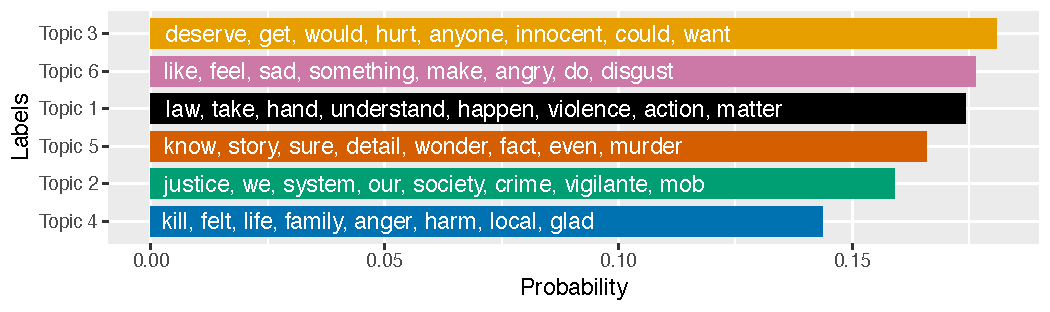
\includegraphics[width=\textwidth]{figures/topic_props.pdf}\\
%\end{figure}\vspace{-2.25em}

%\begin{figure}[H]
%  \caption{Topic Effects by Treatment Group}
%  \centering
%  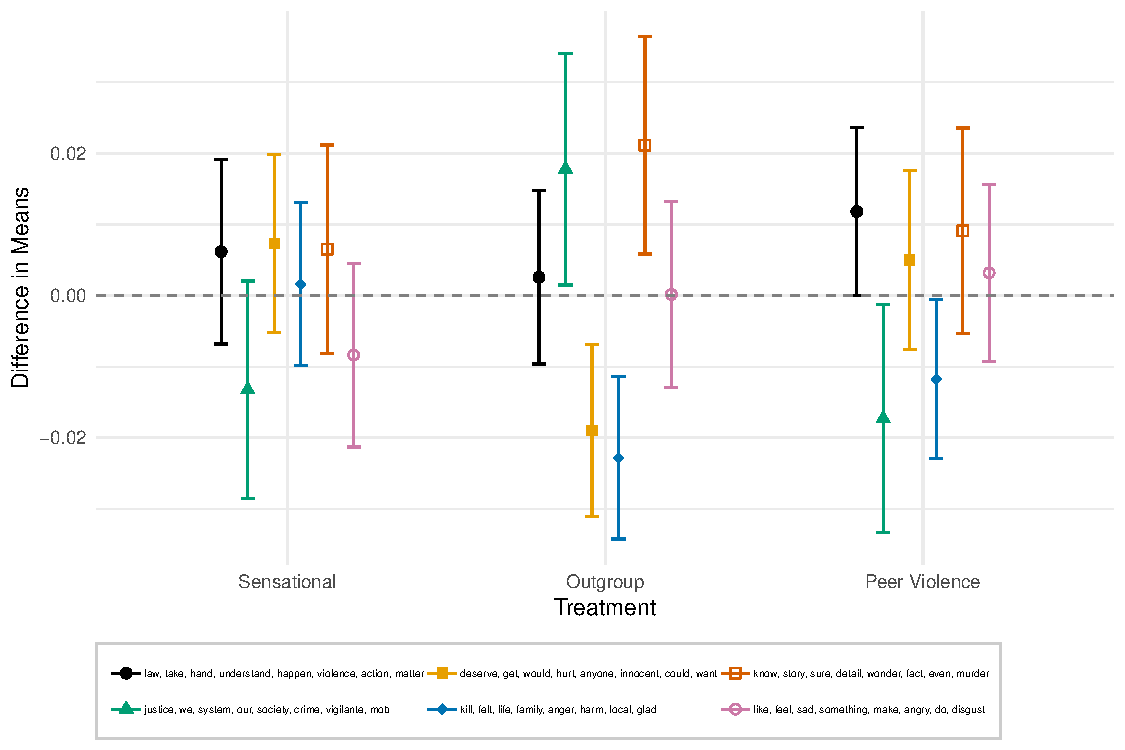
\includegraphics[width=\textwidth]{figures/topic_effects.pdf}\\
%\end{figure}

%\begin{table}[H]
%  \setstretch{1.5}
%  \centering
%  \caption{Most Representative Responses by Topic}
%  \vspace{1em}
%  \resizebox{\textwidth}{!}{
%  \begin{tabular}{|p{.075\textwidth}|p{.8\textwidth}|p{.05\textwidth}|p{.05\textwidth}|p{.05\textwidth}|}
%	\hline
%    \textbf{Topic} & \textbf{Text} & \textbf{Peer} & \textbf{Sens.} & \textbf{Out.} \\\hline
%    Topic 1 & The loss of a child, especially by violence, is unthinkable. I understand the frustration of the locals but vigilante justice is equally unthinkable.  taking the law into one's own hands is despicable. Vigilante justice is never warranted and is horrible. It is outlawed for a reason. & Yes & No & No \\ \hline
%    Topic 2 & Child murderers are some of the worst scum this world can produce. Murderes of any kind are terrible but people that prey on the weakest and most vulnerable aspects of our society are at the bottom of the sludge pit. This man needs to be tried and convicted. A frothing mob cannot be expected to make rational choices and lynching someone in the street is garbage we used to do hundreds of years ago and garbage that third world hellholes continue to do today. I understand being enraged but let the police do their work. & No & No & No \\ \hline
%    Topic 3 & the man got what he deserved. he should get more than that though. anyone who hurts a child should get the strictest punishment he got what he deserved. no one should hurt an innocent defenseless child & Yes & No & Yes \\ \hline
%    Topic 4 & I felt anger and fear. I felt extreme sadness for the victim and the victim's family. I feel confusion about something like this could happen. I felt the attack of the perpetrator were justified. It was only a small step of vindication that the victim and the victim's family deserve. & No & Yes & Yes \\ \hline
%    Topic 5 & As noted in my comment regarding the article provided, there is far too little detail to draw any conclusions regarding the incident other than it is profoundly horrific and sad.  I have many questions to be answered to even begin to form a cohesive assessment of this tragedy. Again, there is not enough information to draw an intelligent conclusion.  One can only presume that the emotional reaction of the bystanders was reactionary and vengeful due to the immediacy of the event. & Yes & Yes & No \\ \hline
%    Topic 6 & I feel like people should not be driven to these extremes. It is a little ridiculous that humans act like this. I hope everyone begins to chill more I feel like he is someone to be punished but if you are to do the same thing as he doing you are no better. To become what others are negatively will ultimately be the same fate. & No & No & Yes \\ \hline
%  \end{tabular}
%  }
%\end{table}

\subsection{Key Words in Open-Ended Outcomes by Treatment Group}

\begin{figure}[H]
  \caption{Key Terms in Sensational Treatment Group}
  \centering
  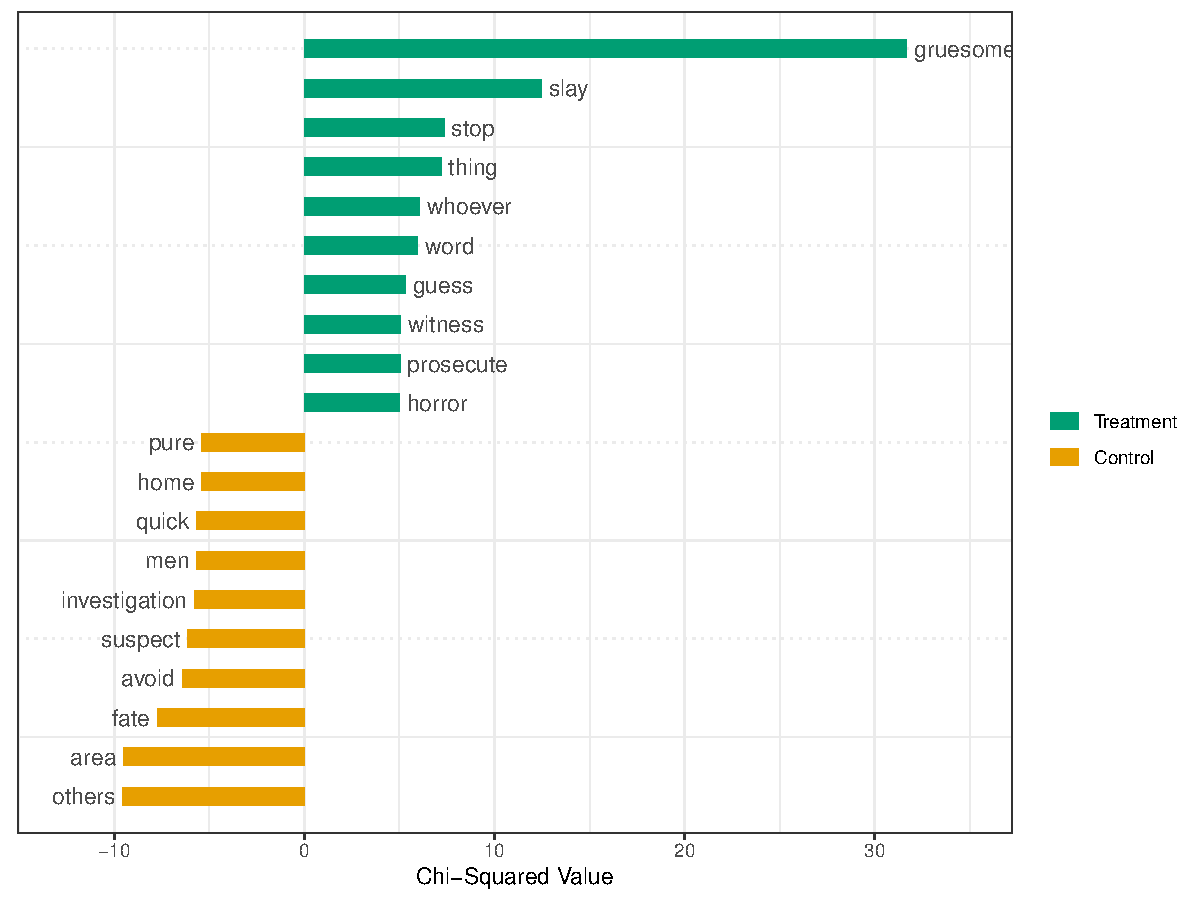
\includegraphics[width=.7\textwidth]{figures/keywords_factor_sensational.pdf}\\
\end{figure}

\begin{figure}[H]
  \caption{Key Terms in Peer Violence Treatment Group}
  \centering
  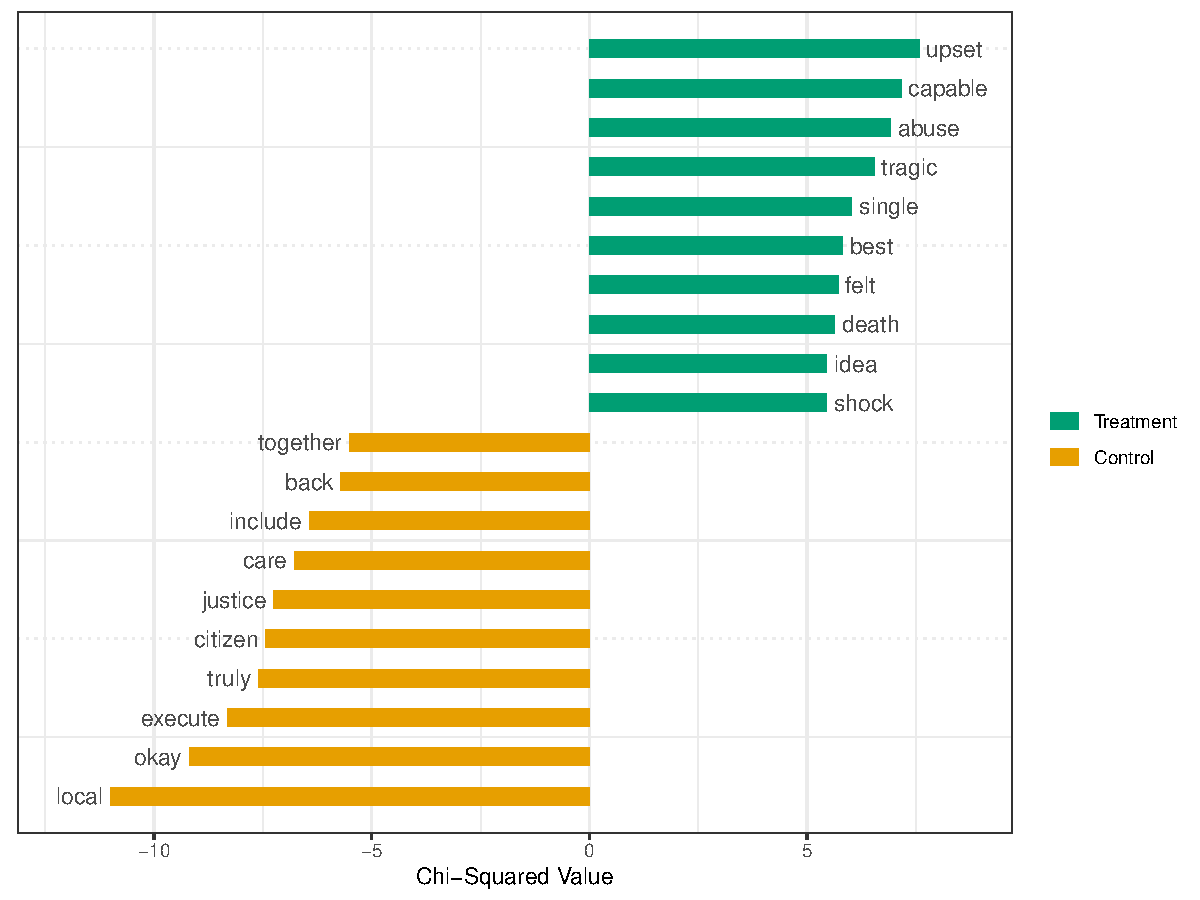
\includegraphics[width=.7\textwidth]{figures/keywords_factor_peer_viol.pdf}\\
\end{figure}

\begin{figure}[H]
  \caption{Key Terms in Outgroup Treatment Group}
  \centering
  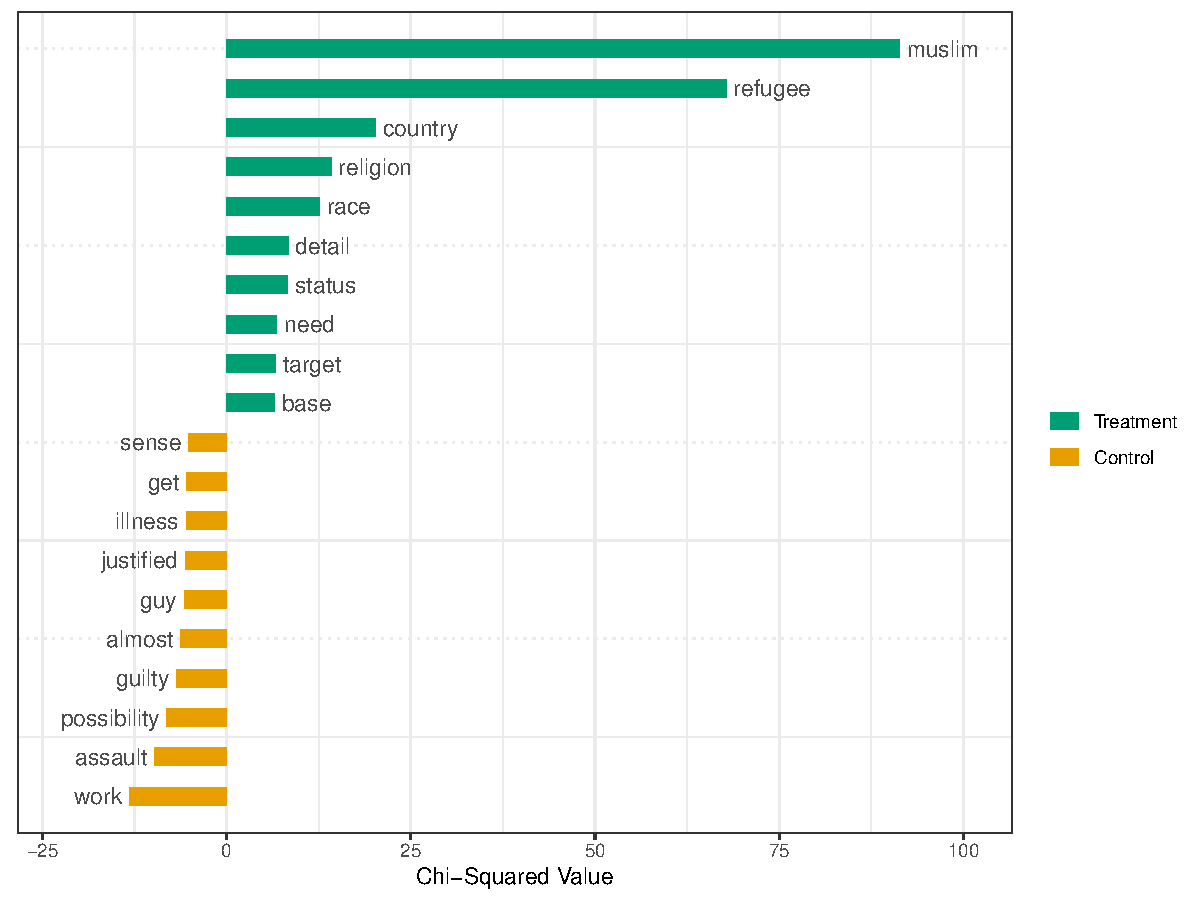
\includegraphics[width=.7\textwidth]{figures/keywords_factor_outgroup.pdf}\\
\end{figure}


\subsection{Open-Ended Outcomes by Treatment Group}


\begin{table}[H] \centering 
  \caption{OLS Model for Expressed Support for Violence, Extrajudicial Violence, and Lethal Violence in Open-ended Responses} 
  \label{} 
\resizebox{\textwidth}{!}{\begin{tabular}{@{\extracolsep{5pt}}lcccccc} 
\\[-1.8ex]\hline 
\hline \\[-1.8ex] 
 & \multicolumn{6}{c}{\textit{Dependent variable:}} \\ 
\cline{2-7} 
 & Violence & Violence & Violence & Extrajudicial Violence & Extrajudicial Violence & Extrajudicial Violence \\ 
\\[-1.8ex] & (1) & (2) & (3) & (4) & (5) & (6)\\ 
\hline \\[-1.8ex] 
 Sensational & 0.057$^{**}$ & 0.063$^{***}$ & 0.063$^{**}$ & 0.052$^{**}$ & 0.057$^{**}$ & 0.056$^{**}$ \\ 
  & (0.025) & (0.024) & (0.024) & (0.024) & (0.023) & (0.023) \\ 
  & & & & & & \\ 
 Outgroup & $-$0.075$^{***}$ & $-$0.192$^{**}$ & $-$0.200$^{**}$ & $-$0.069$^{***}$ & $-$0.148$^{*}$ & $-$0.149$^{*}$ \\ 
  & (0.025) & (0.084) & (0.083) & (0.024) & (0.080) & (0.079) \\ 
  & & & & & & \\ 
 Peer Violence & $-$0.036 & $-$0.035 & $-$0.035 & $-$0.009 & $-$0.009 & $-$0.008 \\ 
  & (0.025) & (0.024) & (0.024) & (0.024) & (0.023) & (0.023) \\ 
  & & & & & & \\ 
 Auth. (Log) &  & 0.048 & 0.047 &  & 0.038 & 0.035 \\ 
  &  & (0.029) & (0.029) &  & (0.030) & (0.029) \\ 
  & & & & & & \\ 
 Ethno. &  & 0.002$^{**}$ &  &  & 0.003$^{***}$ &  \\ 
  &  & (0.001) &  &  & (0.001) &  \\ 
  & & & & & & \\ 
 Anti-Muslim Sentiment &  &  & 0.002$^{***}$ &  &  & 0.003$^{***}$ \\ 
  &  &  & (0.001) &  &  & (0.001) \\ 
  & & & & & & \\ 
 Symb. Racism (Log) &  & 0.053 & 0.050 &  & 0.061 & 0.050 \\ 
  &  & (0.052) & (0.052) &  & (0.053) & (0.052) \\ 
  & & & & & & \\ 
 South &  & 0.051$^{**}$ & 0.049$^{*}$ &  & 0.062$^{**}$ & 0.058$^{**}$ \\ 
  &  & (0.025) & (0.025) &  & (0.025) & (0.024) \\ 
  & & & & & & \\ 
 Republican &  & 0.073$^{**}$ & 0.069$^{**}$ &  & 0.088$^{***}$ & 0.083$^{***}$ \\ 
  &  & (0.030) & (0.030) &  & (0.031) & (0.030) \\ 
  & & & & & & \\ 
 Outgroup x Auth. (Log) &  & 0.015 & 0.013 &  & 0.047 & 0.045 \\ 
  &  & (0.041) & (0.041) &  & (0.041) & (0.040) \\ 
  & & & & & & \\ 
 Outgroup x Ethno &  & $-$0.001 &  &  & $-$0.0005 &  \\ 
  &  & (0.001) &  &  & (0.001) &  \\ 
  & & & & & & \\ 
 Outgroup x Anti-Muslim Sentiment &  &  & $-$0.0002 &  &  & $-$0.0003 \\ 
  &  &  & (0.001) &  &  & (0.001) \\ 
  & & & & & & \\ 
 Outgroup x Symb. Racism (Log) &  & 0.110 & 0.099 &  & 0.050 & 0.048 \\ 
  &  & (0.072) & (0.072) &  & (0.071) & (0.071) \\ 
  & & & & & & \\ 
\hline \\[-1.8ex] 
Observations & 1,613 &  &  & 1,613 &  &  \\ 
\hline 
\hline \\[-1.8ex] 
\textit{Note:}  & \multicolumn{6}{r}{$^{*}$p$<$0.1; $^{**}$p$<$0.05; $^{***}$p$<$0.01} \\ 
\end{tabular}} 
\end{table} 


%\subsection{Log Odds of Terms by Treatment Group}

%To summarize key terms that are most predictive of the treatments experienced by the author, we ran 1000 $\ell_2$ normalized logistic regression models on bootstrap samples of our data. The outcome of each model was the binary treatment indicator and predictors were spelling-corrected, lemmatized unigrams to 5-grams of all words in the vocabulary that appeared in more than 5 open-ended responses. By bootstrapping these coefficient estimates, we mitigate the problem of arbitrary shrinkage of one collinear term over the other. Figures 5 to 7 show the distributions of the 25 largest and 25 smallest coefficients that are significant at the $p = .05$ level. These represent the terms that are most predictive of the treatment assignment.

%\begin{figure}[H]
%  \caption{Log Odds of Terms in Sensational Treatment Group}
%  \centering
%  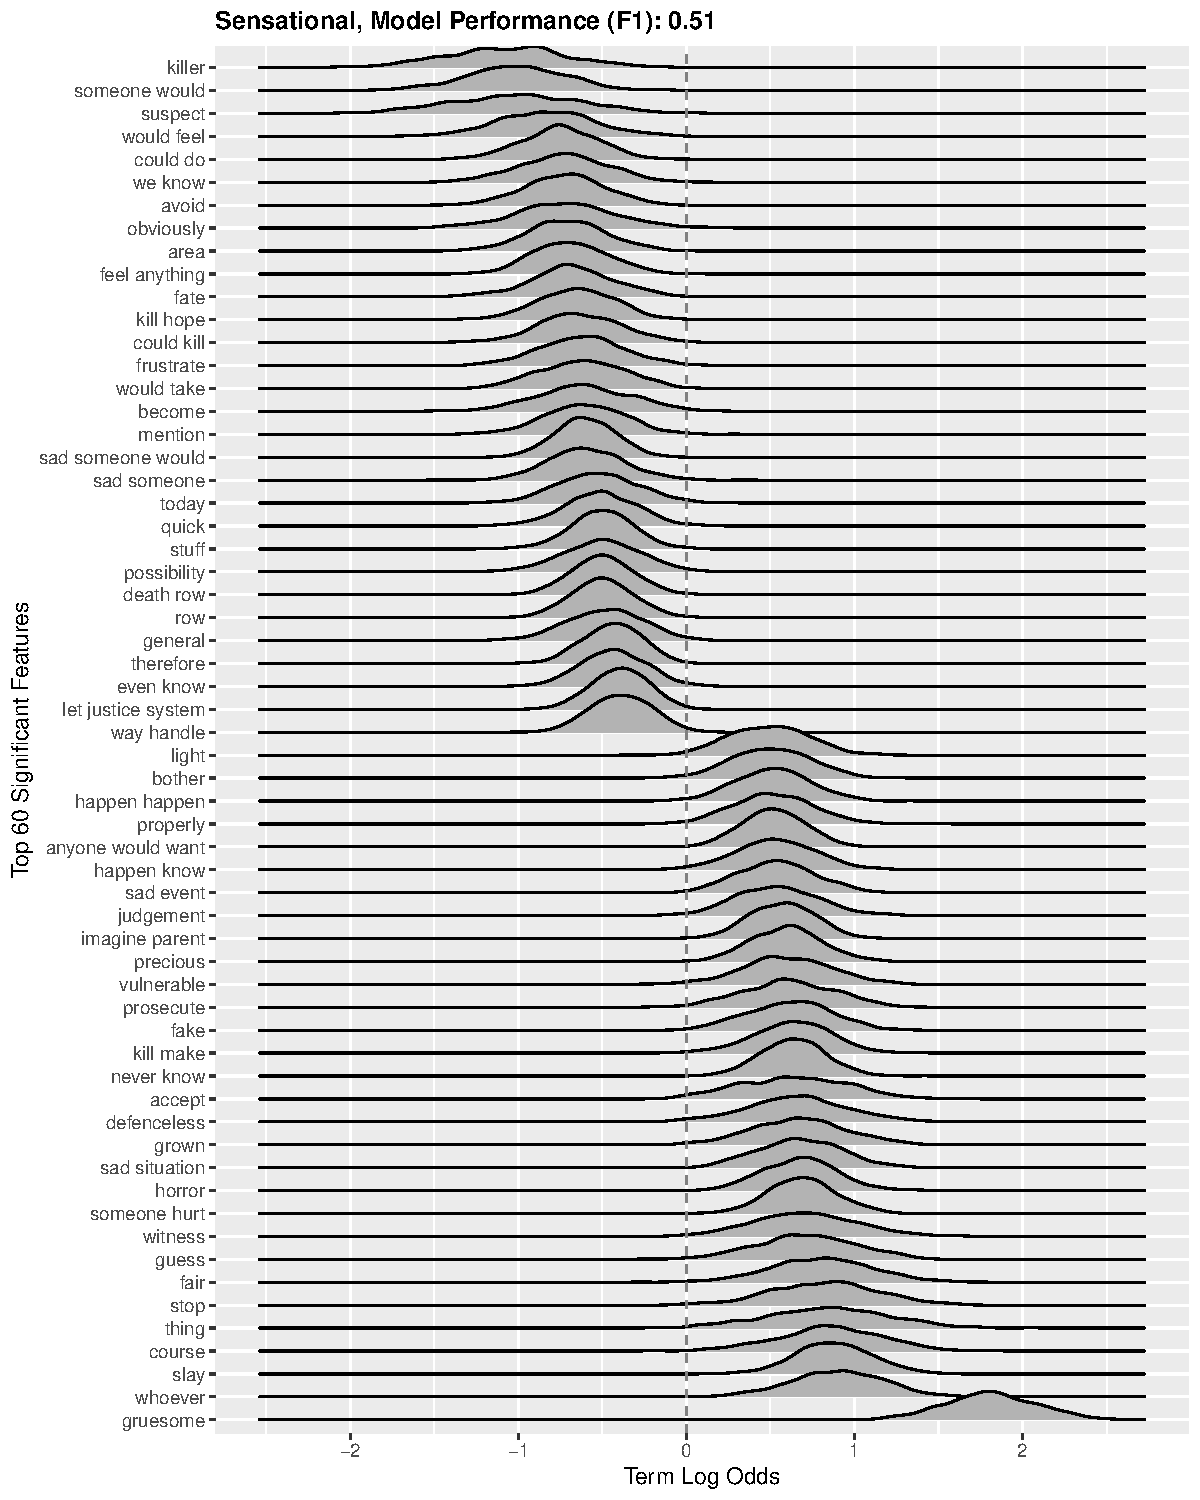
\includegraphics[width=.92\textwidth]{figures/factor_sensational_terms.pdf}\\
%\end{figure}

%\begin{figure}[H]
%  \caption{Log Odds of Terms in Peer Violence Treatment Group}
%  \centering
%  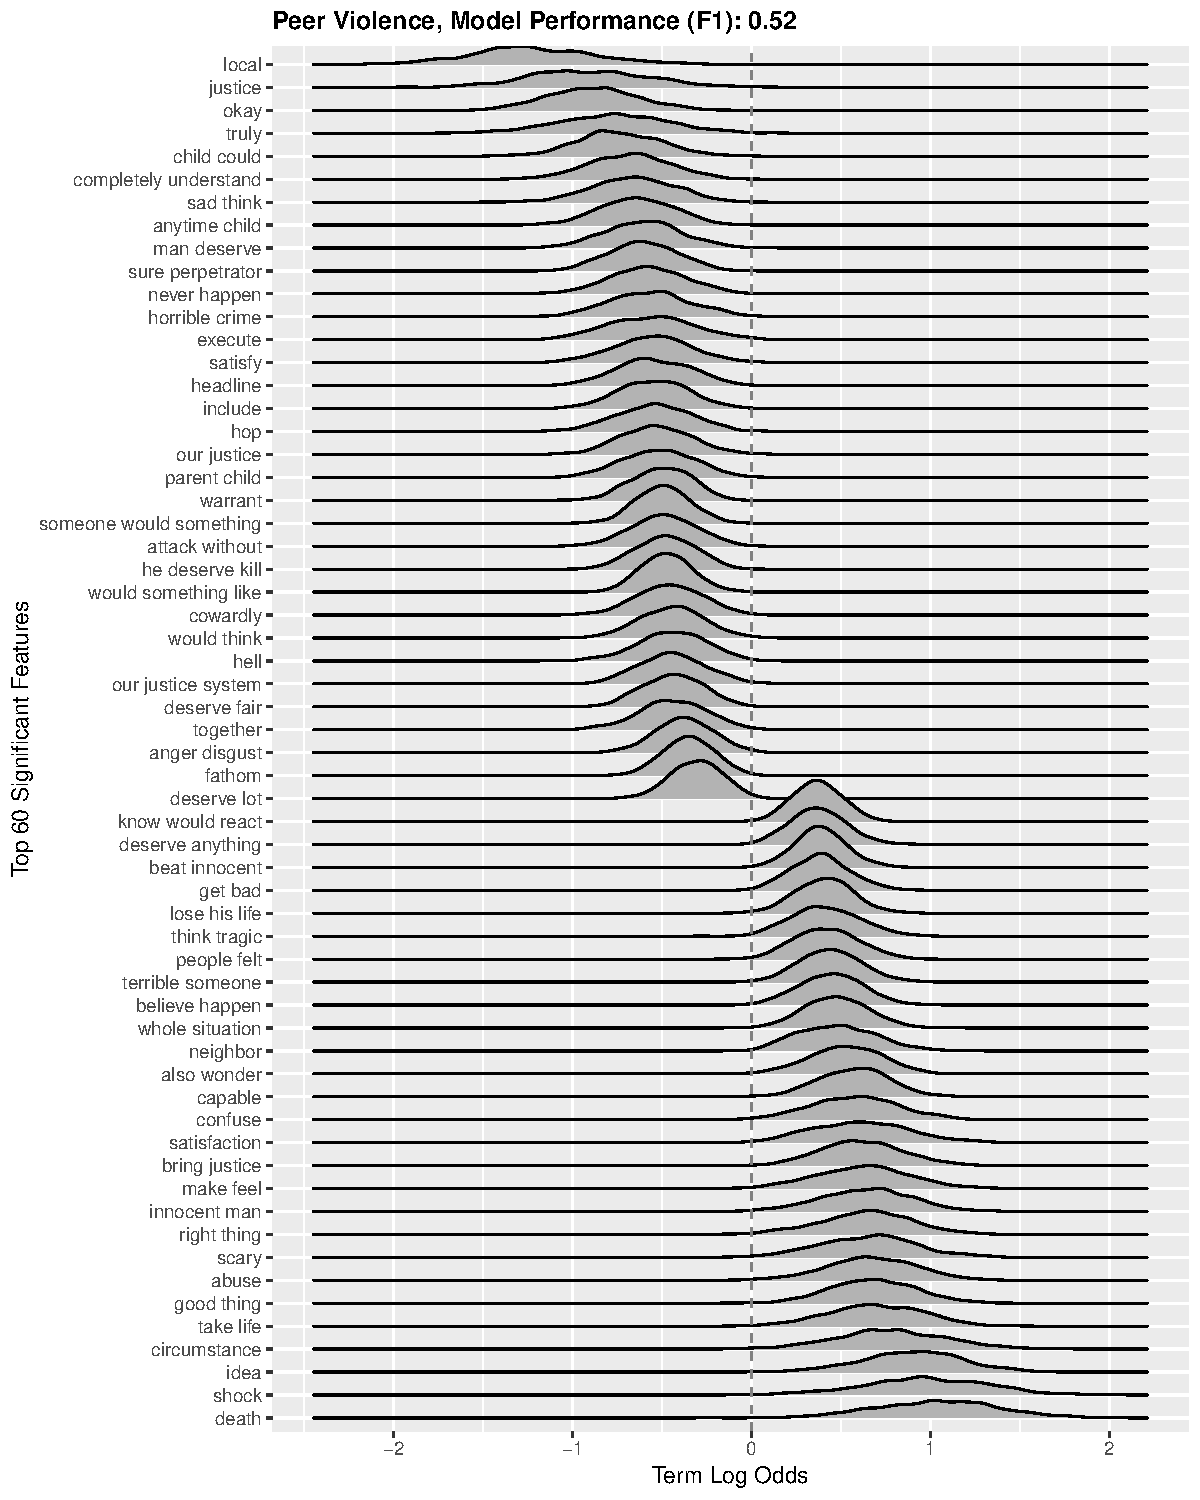
\includegraphics[width=\textwidth]{figures/factor_peer_viol_terms.pdf}\\
%\end{figure}

%\begin{figure}[H]
%  \caption{Log Odds of Terms in Outgroup Treatment Group}
%  \centering
%  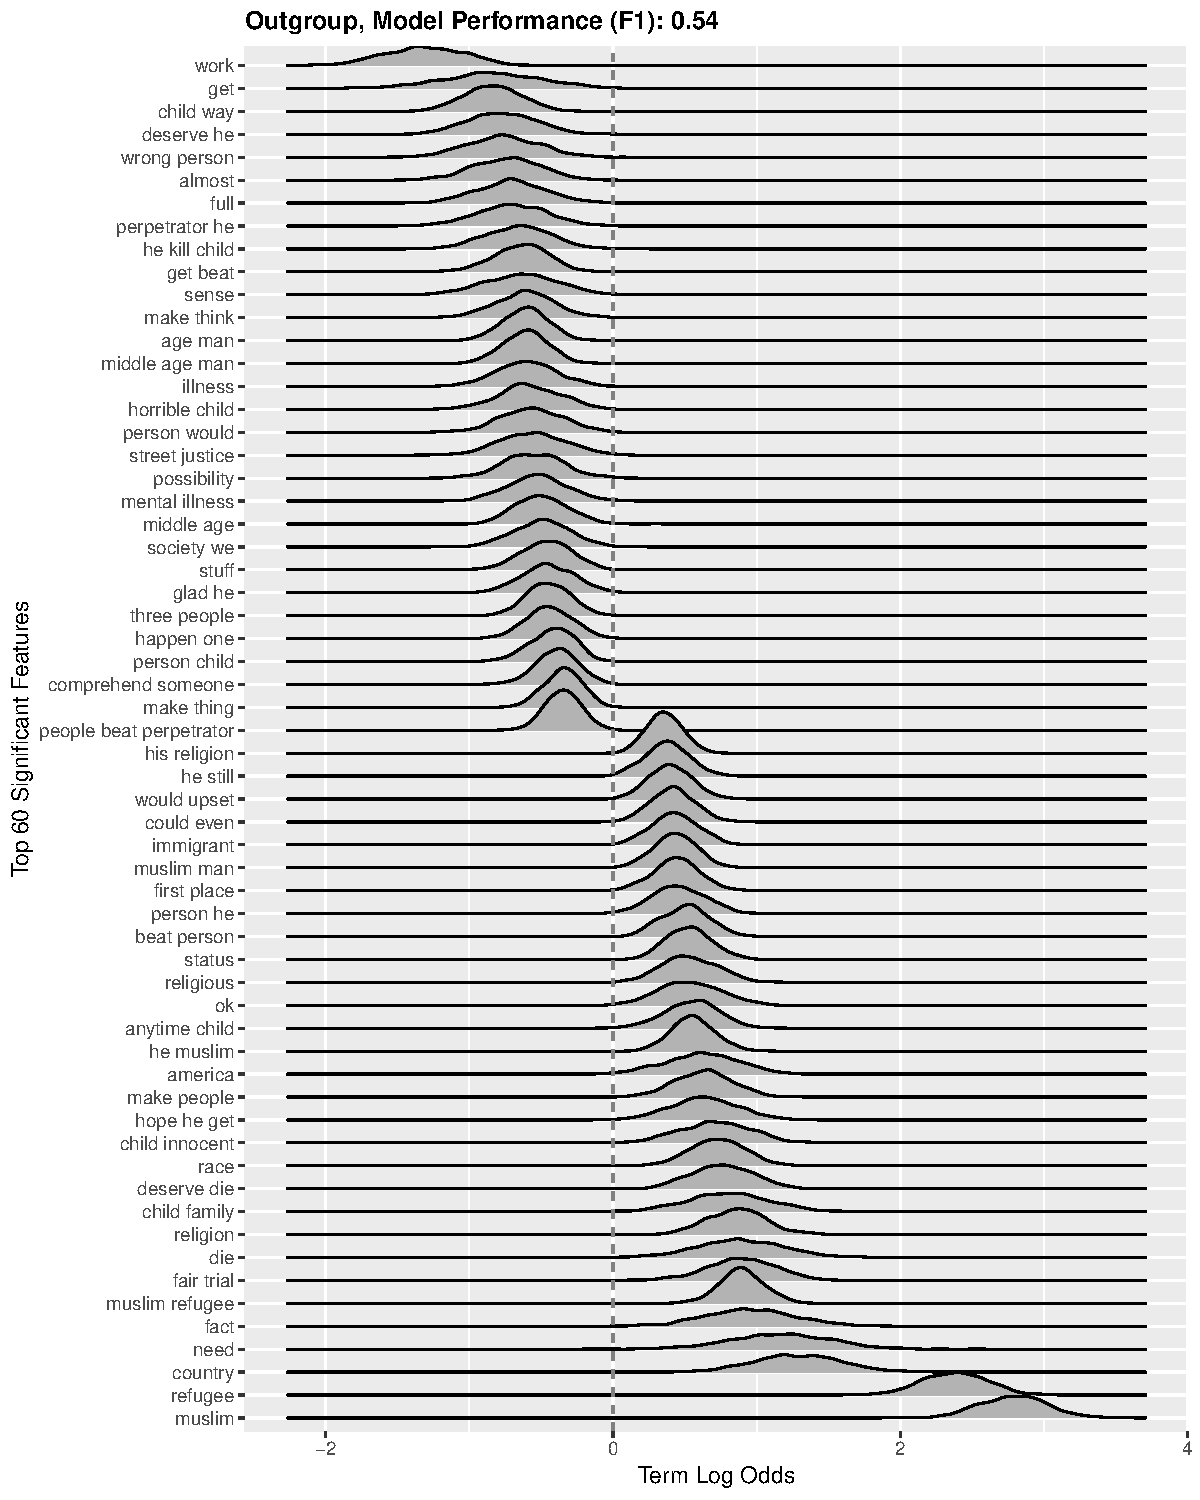
\includegraphics[width=\textwidth]{figures/factor_outgroup_terms.pdf}\\
%\end{figure}

\subsection{Example Open-ended Responses by Condition}

\begin{enumerate}
    \item \textbf{Extrajudicial Violence and Lethal Violence (Outgroup Baseline, Sensational Treatment, Peer-Violence Treatment)}: ``I am absolutely disgusted, appalled, and at a loss for words about this attack. They should kill him in the street. Let everyone who wants a piece of him have a piece of him.''
    \item \textbf{Lethal Violence (Outgroup Treatment, Sensational Treatment, Peer-Violence Baseline)}: ``I think the perpetrator got what he deserved.  It is a shame that they didn't kill him the same way he killed the child.  The attackers shouldn't be punished for attacking the perpetrator.''
    \item \textbf{Judicial Violence (Outgroup Treatment, Sensational Treatment, Peer-Violence Baseline)}: ``Horrible that anyone would want to harm or kill a child. Worst of the worst in society. They should be punished to the fullest extent by the laws.''
    \item \textbf{Information-Seeking (Outgroup Treatment, Sensational Baseline, Peer Violence Baseline)}: ``I want to know what happened. I want to know if the person that was beat up is the one accused of the murder. I want to know the details''
    \item \textbf{Information-Seeking (Outgroup Baseline, Sensational Baseline, Peer-Violence Treatment)}: ``I wanted to know more behind it.  My reaction was what happened.  The article only stated that a homicide had occurred to a child and that the victim's identity as well as the perpetrator's identity hadn't been released, but there were not circumstances stated around the incident.''
    \item \textbf{Cognitive Dissonance (Outgroup Treatment, Sensational Treatment, Peer-Violence Treatment)}: ``It's weird because just not knowing the details, just gut reaction I feel good that the mofo got what he deserved but then I start thinking more and I really don't know any details and the alleged perpetrator has not been convicted. I'm conflicted''
    \item \textbf{Racism (Outgroup Treatment, Sensational Control, Peer-Violence Treatment)}: ``I wonder if, because he was Muslim, he was unjustly targeted. There didn't seem to be any proof yet of who was responsible. I never agree with using violence to address a violent act.''
    \item \textbf{Cognitive Dissonance and Racism (Outgroup Treatment, Sensational Treatment, Peer-Violence Treatment)}: ``I was originally thinking "good for them". Then I thought "what if that dude didn't do it and they angry mob just beat up a muslim. Then I felt remorse for the whole situation. ''
    \item \textbf{Surprise at Lack of Emotion in Article (Outgroup Treatment, Sensational Baseline, Peer-Violence Baseline)}: ``That's one of the most unemotionally written articles I've came across in quiet a while. Most articles are written in a way to elicit feelings of emotion from it's audience. The behavior of the accused is deplorable but the author didn't present it that way. It seemed to be more focused on the attack against the accused.''
\end{enumerate}

\subsection{Example Comments by Condition}

\begin{enumerate}
    \item \textbf{Judicial Violence (Outgroup Treatment, Sensational Baseline, Peer-Violence Treatment)}: ``This middle-aged male Muslim refugee who had been living in the community for about one year should be sent back to where he came from and let them deal with him. This person is not going to last very long in prison.''
    \item \textbf{Judicial and Lethal Violence (Outgroup Baseline, Sensational Baseline, Peer-Violence Treatment)}: ``I think this person should get death penalty for killing a child.''
    \item \textbf{Lethal Violence (Outgroup Baseline, Sensational Treatment, Peer-Violence Baseline)}: ``They should have killed him right then and there. Hopefully they put him in general population and do not waste tax money protecting him from other inmates.''
    \item \textbf{Racism (Outgroup Treatment, Sensational Treatment, Peer-Violence Treatment)}: ``This is clearly a hate crime. There's no mention of evidence, since of course they didn't need any to savagely beat a Muslim refugee. This is just more right-wing paranoia, racism, and violence.''
    \item \textbf{Concerns with Vigilantism (Outgroup Baseline, Sensational Baseline, Peer-Violence Treatment)} ``We should be wary about rushing to judgment.  The murder of a child is a most heinous crime, but unless someone actually witnessed it happen or has incontrovertible proof it is possible that the suspect is actually innocent.  If that is the case then it would turn out that the local residents beat up an innocent man, while the real murderer is out there.'' 
    \item \textbf{Demonizing (Outgroup Baseline, Sensational Treatment, Peer-Violence Treatment)} ``What is wrong with him? Who can be so cruel!'' 
    \item \textbf{Dehumanizing and Extrajudicial Violence (Outgroup Baseline, Sensational Baseline, Peer-Violence Treatment)} ``Vigilante justice is the best kind of justice for monsters like this perpetrator!'' 
\end{enumerate}
\newpage

\section{Comments}

%\subsection{Comment Likes}

%\begin{figure}[H]
%  \caption{Bootstrap Proportions of Violent Comment Likes by Treatment Group}\vspace{.5em}
%  \centering
%  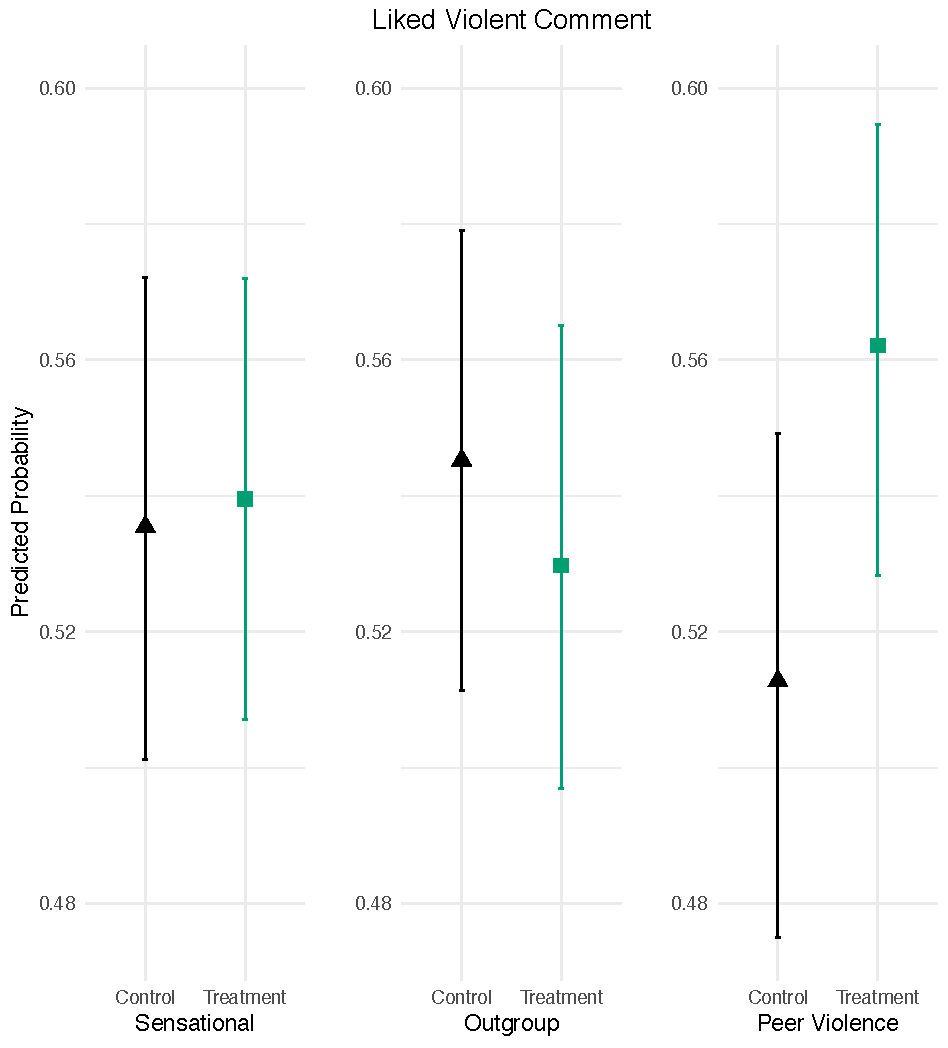
\includegraphics[width=.94\textwidth]{figures/com_viol_like.pdf}\\
%\end{figure}

%\begin{figure}[H]
%  \caption{Bootstrap Proportions of Positive/Conciliatory Comment Likes by Treatment Group}\vspace{.5em}
%  \centering
%  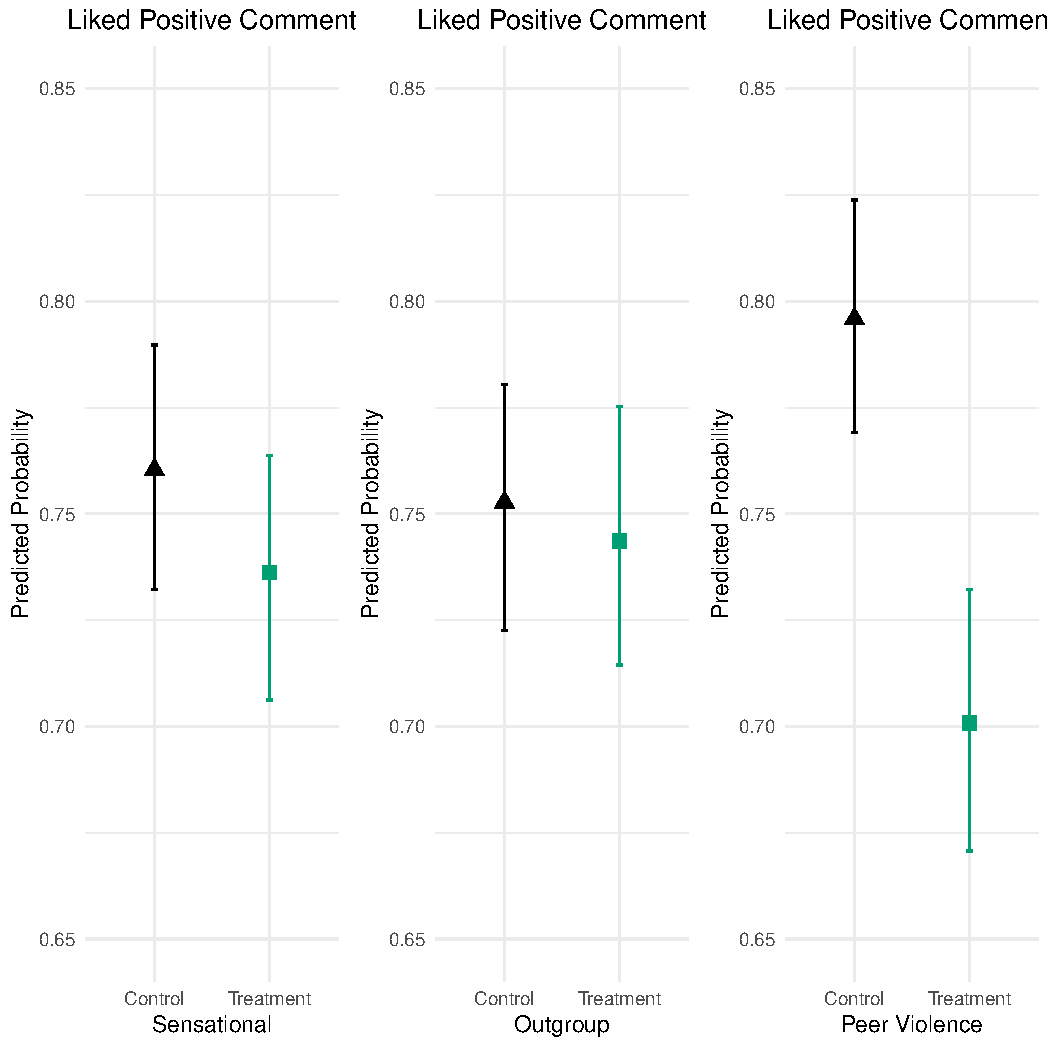
\includegraphics[width=.94\textwidth]{figures/com_pos_like.pdf}\\
%\end{figure}

%\begin{figure}[H]
%  \caption{Bootstrap Proportions of Information-Seeking Comment Likes by Treatment Group}\vspace{.5em}
%  \centering
%  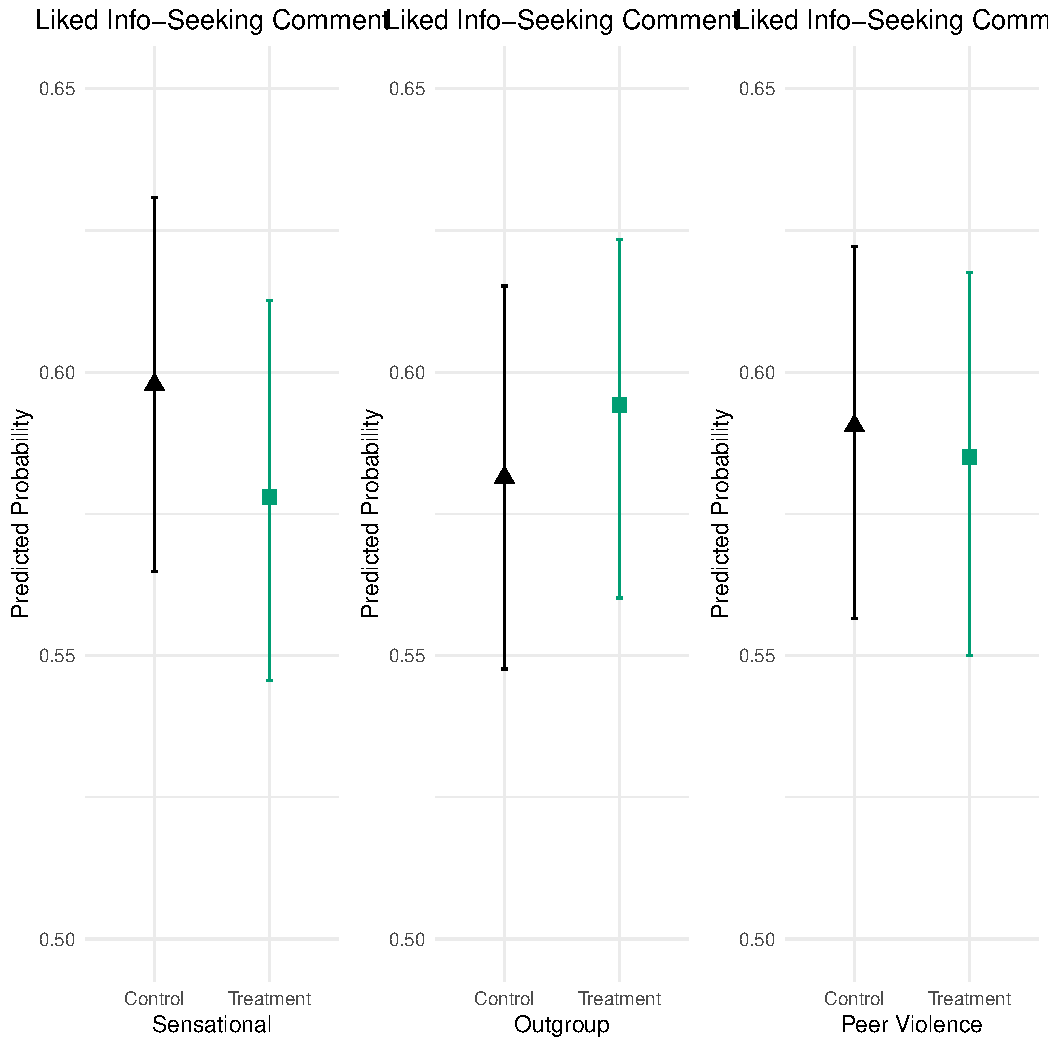
\includegraphics[width=.94\textwidth]{figures/com_info_like.pdf}\\
%\end{figure}

\subsection{Comment Text Models}
{\setstretch{1.25}

\begin{table}[H] \centering 
  \caption{OLS Model for Propensity to Post a Comment} 
  \label{} 
\begin{tabular}{@{\extracolsep{5pt}}lccc} 
\\[-1.8ex]\hline 
\hline \\[-1.8ex] 
 & \multicolumn{3}{c}{\textit{Dependent variable:}} \\ 
\cline{2-4} 
 & Posted a Comment & Posted a Comment & Posted a Comment \\ 
\\[-1.8ex] & (1) & (2) & (3)\\ 
\hline \\[-1.8ex] 
 Sensational & 0.045$^{**}$ & 0.050$^{**}$ & 0.050$^{**}$ \\ 
  & (0.023) & (0.023) & (0.023) \\ 
  & & & \\ 
 Outgroup & $-$0.006 & $-$0.085 & $-$0.080 \\ 
  & (0.023) & (0.080) & (0.079) \\ 
  & & & \\ 
 Peer Violence & 0.027 & 0.026 & 0.026 \\ 
  & (0.023) & (0.023) & (0.023) \\ 
  & & & \\ 
 Auth. (Log) &  & $-$0.002 & $-$0.002 \\ 
  &  & (0.028) & (0.028) \\ 
  & & & \\ 
 Ethno. &  & $-$0.001 &  \\ 
  &  & (0.001) &  \\ 
  & & & \\ 
 Anti-Muslim Sentiment &  &  & $-$0.001 \\ 
  &  &  & (0.001) \\ 
  & & & \\ 
 Symb. Racism (Log) &  & 0.059 & 0.057 \\ 
  &  & (0.049) & (0.049) \\ 
  & & & \\ 
 South &  & 0.007 & 0.007 \\ 
  &  & (0.024) & (0.024) \\ 
  & & & \\ 
 Republican &  & 0.006 & 0.006 \\ 
  &  & (0.029) & (0.029) \\ 
  & & & \\ 
 Outgroup x Auth. (Log) &  & $-$0.005 & $-$0.006 \\ 
  &  & (0.038) & (0.038) \\ 
  & & & \\ 
 Outgroup x Ethno &  & 0.001 &  \\ 
  &  & (0.001) &  \\ 
  & & & \\ 
 Outgroup x Anti-Muslim Sentiment &  &  & 0.001 \\ 
  &  &  & (0.001) \\ 
  & & & \\ 
 Outgroup x Symb. Racism (Log) &  & 0.027 & 0.027 \\ 
  &  & (0.068) & (0.068) \\ 
  & & & \\ 
\hline \\[-1.8ex] 
Observations & 1,652 &  &  \\ 
\hline 
\hline \\[-1.8ex] 
\textit{Note:}  & \multicolumn{3}{r}{$^{*}$p$<$0.1; $^{**}$p$<$0.05; $^{***}$p$<$0.01} \\ 
\end{tabular} 
\end{table} 


\begin{table}[H] \centering 
  \caption{Logit Model for Propensity to Post a Comment} 
  \label{} 
\begin{tabular}{@{\extracolsep{5pt}}lc} 
\\[-1.8ex]\hline 
\hline \\[-1.8ex] 
 & \multicolumn{1}{c}{\textit{Dependent variable:}} \\ 
\cline{2-2} 
 & Posted a Comment \\ 
\hline \\[-1.8ex] 
 Gender & 0.113 \\ 
  & (0.109) \\ 
  & \\ 
 Age & 0.701 \\ 
  & (0.922) \\ 
  & \\ 
 Education & 0.009$^{*}$ \\ 
  & (0.005) \\ 
  & \\ 
 Authoritarian (Log) & 0.042 \\ 
  & (0.042) \\ 
  & \\ 
 Ethnocentrism (Log) & 0.015 \\ 
  & (0.094) \\ 
  & \\ 
 Symbolic Racism (Log) & $-$0.001 \\ 
  & (0.003) \\ 
  & \\ 
 South & 0.305$^{*}$ \\ 
  & (0.175) \\ 
  & \\ 
 Republican & 0.024 \\ 
  & (0.111) \\ 
  & \\ 
 pi\_R & $-$0.002 \\ 
  & (0.135) \\ 
  & \\ 
\hline \\[-1.8ex] 
Observations & 1,655 \\ 
\hline 
\hline \\[-1.8ex] 
\textit{Note:}  & \multicolumn{1}{r}{$^{*}$p$<$0.1; $^{**}$p$<$0.05; $^{***}$p$<$0.01} \\ 
\end{tabular} 
\end{table} 


\begin{table}[H] \centering 
  \caption{Heckman 2-Step Selection Model OLS Model for Expressed Support for Violence, Extrajudicial Violence, and Lethal Violence in Comments} 
  \label{} 
\begin{tabular}{@{\extracolsep{5pt}}lc} 
\\[-1.8ex]\hline 
\hline \\[-1.8ex] 
 & \multicolumn{1}{c}{\textit{Dependent variable:}} \\ 
\cline{2-2} 
 & Violence \\ 
\hline \\[-1.8ex] 
 Sensational & 0.047 \\ 
  & (0.037) \\ 
  & \\ 
 Outgroup & $-$0.063$^{*}$ \\ 
  & (0.036) \\ 
  & \\ 
 Peer Violence & 0.082$^{**}$ \\ 
  & (0.037) \\ 
  & \\ 
\hline \\[-1.8ex] 
Observations & 1,650 \\ 
$\rho$ & $-$0.011 \\ 
Inverse Mills Ratio & $-$0.004  (0.238) \\ 
\hline 
\hline \\[-1.8ex] 
\textit{Note:}  & \multicolumn{1}{r}{$^{*}$p$<$0.1; $^{**}$p$<$0.05; $^{***}$p$<$0.01} \\ 
\end{tabular} 
\end{table} 
}

\begin{landscape}

\begin{table}[H] \centering 
  \caption{Additional Text Responses (Comments)} 
  \label{} 
\resizebox{\textwidth}{!}{\begin{tabular}{@{\extracolsep{5pt}}lcccccccccccc} 
\\[-1.8ex]\hline 
\hline \\[-1.8ex] 
 & \multicolumn{12}{c}{\textit{Dependent variable:}} \\ 
\cline{2-13} 
 & Cognitive Dissonance & Cognitive Dissonance & Cognitive Dissonance & Info. Seeking & Info. Seeking & Info. Seeking & Fake News & Fake News & Fake News & Racism & Racism & Racism \\ 
\\[-1.8ex] & (1) & (2) & (3) & (4) & (5) & (6) & (7) & (8) & (9) & (10) & (11) & (12)\\ 
\hline \\[-1.8ex] 
 Sensational & 0.022 & 0.022 & 0.022 & $-$0.042 & $-$0.044$^{*}$ & $-$0.044$^{*}$ & $-$0.009 & $-$0.009 & $-$0.009 & $-$0.006 & $-$0.012 & $-$0.012 \\ 
  & (0.019) & (0.021) & (0.021) & (0.026) & (0.026) & (0.026) & (0.006) & (0.006) & (0.006) & (0.016) & (0.015) & (0.015) \\ 
  & & & & & & & & & & & & \\ 
 Outgroup & $-$0.007 & $-$0.005 & $-$0.011 & 0.009 & $-$0.050 & $-$0.055 & $-$0.007 & $-$0.008 & $-$0.010 & 0.056$^{***}$ & 0.212$^{***}$ & 0.211$^{***}$ \\ 
  & (0.019) & (0.072) & (0.071) & (0.026) & (0.096) & (0.095) & (0.006) & (0.026) & (0.024) & (0.016) & (0.066) & (0.065) \\ 
  & & & & & & & & & & & & \\ 
 Peer Violence & 0.032$^{*}$ & 0.033$^{*}$ & 0.034$^{*}$ & $-$0.034 & $-$0.034 & $-$0.034 & 0.007 & 0.007 & 0.007 & $-$0.023 & $-$0.019 & $-$0.019 \\ 
  & (0.019) & (0.020) & (0.020) & (0.026) & (0.026) & (0.027) & (0.006) & (0.005) & (0.005) & (0.016) & (0.015) & (0.015) \\ 
  & & & & & & & & & & & & \\ 
 Auth. (Log) &  & $-$0.011 & $-$0.010 &  & $-$0.028 & $-$0.026 &  & 0.005 & 0.005 &  & 0.011 & 0.011 \\ 
  &  & (0.026) & (0.026) &  & (0.028) & (0.028) &  & (0.004) & (0.004) &  & (0.010) & (0.010) \\ 
  & & & & & & & & & & & & \\ 
 Ethno. &  & 0.0004 &  &  & 0.001 &  &  & 0.0003 &  &  & $-$0.0001 &  \\ 
  &  & (0.0005) &  &  & (0.001) &  &  & (0.001) &  &  & (0.0001) &  \\ 
  & & & & & & & & & & & & \\ 
 Anti-Muslim Sentiment &  &  & $-$0.0001 &  &  & $-$0.0001 &  &  & 0.0002 &  &  & $-$0.0001 \\ 
  &  &  & (0.0004) &  &  & (0.001) &  &  & (0.0004) &  &  & (0.0001) \\ 
  & & & & & & & & & & & & \\ 
 Symb. Racism (Log) &  & $-$0.008 & 0.0001 &  & $-$0.086 & $-$0.069 &  & $-$0.019 & $-$0.017 &  & 0.018 & 0.019 \\ 
  &  & (0.032) & (0.032) &  & (0.057) & (0.056) &  & (0.014) & (0.013) &  & (0.014) & (0.014) \\ 
  & & & & & & & & & & & & \\ 
 South &  & 0.031 & 0.031 &  & $-$0.055$^{**}$ & $-$0.058$^{**}$ &  & $-$0.005 & $-$0.006 &  & $-$0.002 & $-$0.002 \\ 
  &  & (0.021) & (0.021) &  & (0.025) & (0.025) &  & (0.004) & (0.004) &  & (0.016) & (0.016) \\ 
  & & & & & & & & & & & & \\ 
 Republican &  & $-$0.006 & $-$0.005 &  & 0.035 & 0.035 &  & 0.007 & 0.007 &  & $-$0.021 & $-$0.020 \\ 
  &  & (0.024) & (0.024) &  & (0.032) & (0.033) &  & (0.007) & (0.007) &  & (0.016) & (0.016) \\ 
  & & & & & & & & & & & & \\ 
 Outgroup x Auth. (Log) &  & 0.006 & 0.006 &  & 0.038 & 0.035 &  & $-$0.005 & $-$0.005 &  & $-$0.018 & $-$0.017 \\ 
  &  & (0.034) & (0.035) &  & (0.043) & (0.043) &  & (0.004) & (0.004) &  & (0.024) & (0.024) \\ 
  & & & & & & & & & & & & \\ 
 Outgroup x Ethno &  & $-$0.001 &  &  & 0.0002 &  &  & $-$0.0003 &  &  & $-$0.0003 &  \\ 
  &  & (0.001) &  &  & (0.001) &  &  & (0.001) &  &  & (0.001) &  \\ 
  & & & & & & & & & & & & \\ 
 Outgroup x Anti-Muslim Sentiment &  &  & $-$0.0005 &  &  & 0.001 &  &  & $-$0.0002 &  &  & $-$0.0004 \\ 
  &  &  & (0.0005) &  &  & (0.001) &  &  & (0.0004) &  &  & (0.001) \\ 
  & & & & & & & & & & & & \\ 
 Outgroup x Symb. Racism (Log) &  & 0.020 & 0.014 &  & 0.024 & 0.006 &  & 0.013 & 0.010 &  & $-$0.103$^{***}$ & $-$0.100$^{**}$ \\ 
  &  & (0.061) & (0.060) &  & (0.077) & (0.078) &  & (0.010) & (0.010) &  & (0.039) & (0.040) \\ 
  & & & & & & & & & & & & \\ 
\hline \\[-1.8ex] 
Observations & 498 &  &  & 498 &  &  & 498 &  &  & 498 &  &  \\ 
\hline 
\hline \\[-1.8ex] 
\textit{Note:}  & \multicolumn{12}{r}{$^{*}$p$<$0.1; $^{**}$p$<$0.05; $^{***}$p$<$0.01} \\ 
\end{tabular}} 
\end{table} 


\begin{table}[H] \centering 
  \caption{Additional Text Responses (Open Ended)} 
  \label{} 
\resizebox{8.5in}{!}{\begin{tabular}{@{\extracolsep{5pt}}lccccccccccccccc} 
\\[-1.8ex]\hline 
\hline \\[-1.8ex] 
 & \multicolumn{15}{c}{\textit{Dependent variable:}} \\ 
\cline{2-16} 
 & Cognitive Dissonance & Cognitive Dissonance & Cognitive Dissonance & Info. Seeking & Info. Seeking & Info. Seeking & Fake News & Fake News & Fake News & Racism & Racism & Racism & Social Desirability & Social Desirability & Social Desirability \\ 
\\[-1.8ex] & (1) & (2) & (3) & (4) & (5) & (6) & (7) & (8) & (9) & (10) & (11) & (12) & (13) & (14) & (15)\\ 
\hline \\[-1.8ex] 
 Sensational & 0.046$^{**}$ & 0.046$^{**}$ & 0.046$^{**}$ & 0.011 & 0.008 & 0.008 & 0.006 & 0.006 & 0.006 & $-$0.007 & $-$0.010 & $-$0.010 & $-$0.001 & $-$0.001 & $-$0.001 \\ 
  & (0.019) & (0.019) & (0.019) & (0.015) & (0.015) & (0.015) & (0.006) & (0.006) & (0.006) & (0.011) & (0.011) & (0.011) & (0.006) & (0.006) & (0.006) \\ 
  & & & & & & & & & & & & & & & \\ 
 Outgroup & $-$0.036$^{*}$ & $-$0.066 & $-$0.068 & 0.020 & 0.011 & 0.005 & $-$0.003 & $-$0.032$^{**}$ & $-$0.033$^{**}$ & 0.080$^{***}$ & 0.169$^{***}$ & 0.169$^{***}$ & 0.031$^{***}$ & 0.028 & 0.028 \\ 
  & (0.019) & (0.069) & (0.068) & (0.015) & (0.055) & (0.054) & (0.006) & (0.016) & (0.017) & (0.011) & (0.044) & (0.044) & (0.006) & (0.018) & (0.018) \\ 
  & & & & & & & & & & & & & & & \\ 
 Peer Violence & 0.004 & 0.003 & 0.003 & 0.002 & 0.001 & 0.001 & 0.003 & 0.003 & 0.003 & $-$0.025$^{**}$ & $-$0.025$^{**}$ & $-$0.025$^{**}$ & $-$0.003 & $-$0.002 & $-$0.002 \\ 
  & (0.019) & (0.019) & (0.019) & (0.015) & (0.015) & (0.015) & (0.006) & (0.006) & (0.006) & (0.011) & (0.011) & (0.011) & (0.006) & (0.006) & (0.006) \\ 
  & & & & & & & & & & & & & & & \\ 
 Auth. (Log) &  & $-$0.047$^{*}$ & $-$0.046$^{*}$ &  & $-$0.049$^{***}$ & $-$0.049$^{***}$ &  & $-$0.017$^{**}$ & $-$0.016$^{**}$ &  & $-$0.004 & $-$0.004 &  & $-$0.001 & $-$0.001 \\ 
  &  & (0.024) & (0.024) &  & (0.017) & (0.017) &  & (0.007) & (0.007) &  & (0.007) & (0.007) &  & (0.001) & (0.001) \\ 
  & & & & & & & & & & & & & & & \\ 
 Ethno. &  & 0.001 &  &  & 0.001$^{*}$ &  &  & 0.0004$^{*}$ &  &  & $-$0.0002 &  &  & 0.00001 &  \\ 
  &  & (0.001) &  &  & (0.001) &  &  & (0.0002) &  &  & (0.0003) &  &  & (0.00001) &  \\ 
  & & & & & & & & & & & & & & & \\ 
 Anti-Muslim Sentiment &  &  & 0.0004 &  &  & 0.001 &  &  & 0.0002 &  &  & $-$0.0002 &  &  & 0.00000 \\ 
  &  &  & (0.001) &  &  & (0.001) &  &  & (0.0002) &  &  & (0.0002) &  &  & (0.00001) \\ 
  & & & & & & & & & & & & & & & \\ 
 Symb. Racism (Log) &  & $-$0.037 & $-$0.032 &  & $-$0.057$^{*}$ & $-$0.055$^{*}$ &  & $-$0.009 & $-$0.007 &  & $-$0.017 & $-$0.016 &  & $-$0.002 & $-$0.002 \\ 
  &  & (0.043) & (0.043) &  & (0.031) & (0.031) &  & (0.010) & (0.010) &  & (0.016) & (0.016) &  & (0.004) & (0.004) \\ 
  & & & & & & & & & & & & & & & \\ 
 South &  & 0.007 & 0.007 &  & $-$0.028$^{*}$ & $-$0.029$^{*}$ &  & $-$0.004 & $-$0.004 &  & $-$0.020$^{*}$ & $-$0.020$^{*}$ &  & 0.002 & 0.002 \\ 
  &  & (0.020) & (0.020) &  & (0.015) & (0.015) &  & (0.006) & (0.006) &  & (0.011) & (0.011) &  & (0.006) & (0.006) \\ 
  & & & & & & & & & & & & & & & \\ 
 Republican &  & $-$0.0004 & $-$0.001 &  & 0.004 & 0.003 &  & $-$0.001 & $-$0.001 &  & 0.002 & 0.002 &  & 0.005 & 0.005 \\ 
  &  & (0.024) & (0.024) &  & (0.018) & (0.018) &  & (0.007) & (0.007) &  & (0.012) & (0.012) &  & (0.009) & (0.009) \\ 
  & & & & & & & & & & & & & & & \\ 
 Outgroup x Auth. (Log) &  & 0.042 & 0.042 &  & 0.022 & 0.022 &  & 0.016$^{*}$ & 0.015$^{*}$ &  & $-$0.046$^{**}$ & $-$0.046$^{**}$ &  & 0.011 & 0.011 \\ 
  &  & (0.032) & (0.032) &  & (0.025) & (0.025) &  & (0.008) & (0.009) &  & (0.019) & (0.019) &  & (0.011) & (0.011) \\ 
  & & & & & & & & & & & & & & & \\ 
 Outgroup x Ethno &  & $-$0.001 &  &  & $-$0.001 &  &  & $-$0.0003 &  &  & 0.0002 &  &  & $-$0.0001 &  \\ 
  &  & (0.001) &  &  & (0.001) &  &  & (0.0003) &  &  & (0.001) &  &  & (0.0003) &  \\ 
  & & & & & & & & & & & & & & & \\ 
 Outgroup x Anti-Muslim Sentiment &  &  & $-$0.0004 &  &  & $-$0.001 &  &  & $-$0.0002 &  &  & 0.0002 &  &  & $-$0.0001 \\ 
  &  &  & (0.001) &  &  & (0.001) &  &  & (0.0002) &  &  & (0.0005) &  &  & (0.0002) \\ 
  & & & & & & & & & & & & & & & \\ 
 Outgroup x Symb. Racism (Log) &  & 0.016 & 0.015 &  & 0.032 & 0.029 &  & 0.022 & 0.022 &  & $-$0.052 & $-$0.051 &  & $-$0.001 & $-$0.001 \\ 
  &  & (0.056) & (0.056) &  & (0.045) & (0.045) &  & (0.015) & (0.015) &  & (0.034) & (0.034) &  & (0.015) & (0.015) \\ 
  & & & & & & & & & & & & & & & \\ 
\hline \\[-1.8ex] 
Observations & 1,623 &  &  & 1,623 &  &  & 1,623 &  &  & 1,623 &  &  & 1,623 &  &  \\ 
\hline 
\hline \\[-1.8ex] 
\textit{Note:}  & \multicolumn{15}{r}{$^{*}$p$<$0.1; $^{**}$p$<$0.05; $^{***}$p$<$0.01} \\ 
\end{tabular}} 
\end{table} 

\end{landscape}

\begin{figure}[!htbp]
  \centering
  \caption{Additional Comment Outcomes by Treatment Condition}
  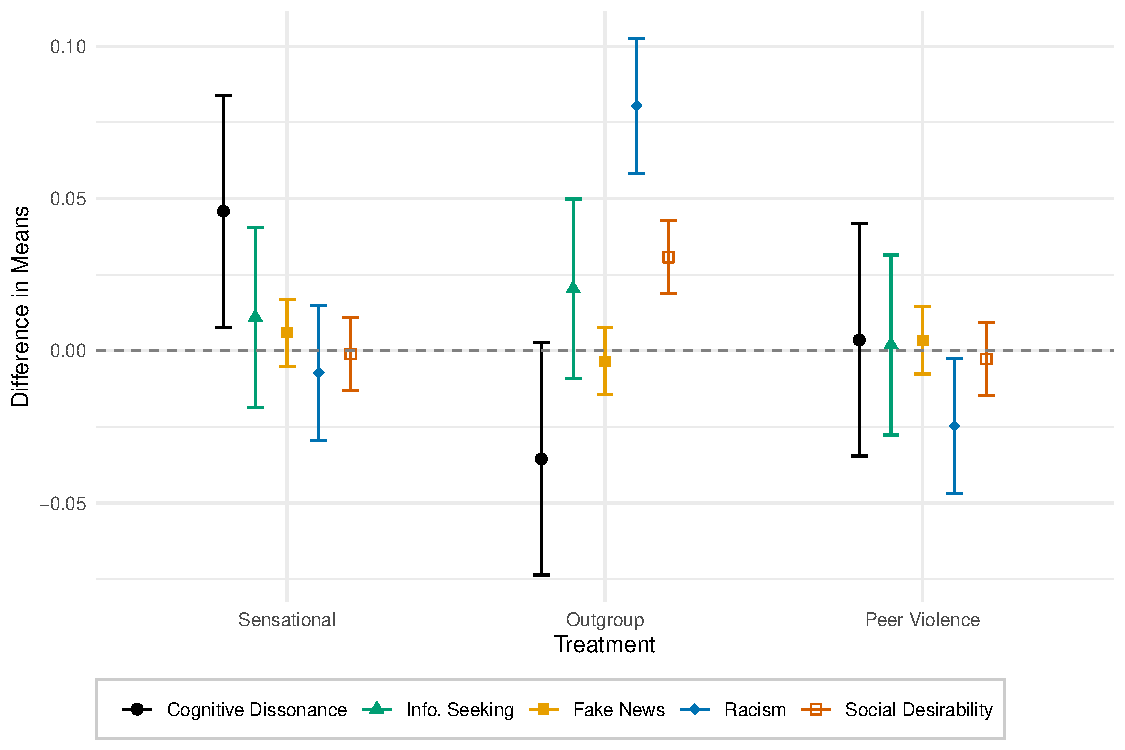
\includegraphics[width=.8\textwidth]{figures/additional_text_oe.pdf}
\end{figure}

\begin{figure}[!htbp]
  \centering
  \caption{Additional Open-Ended Outcomes by Treatment Condition}
  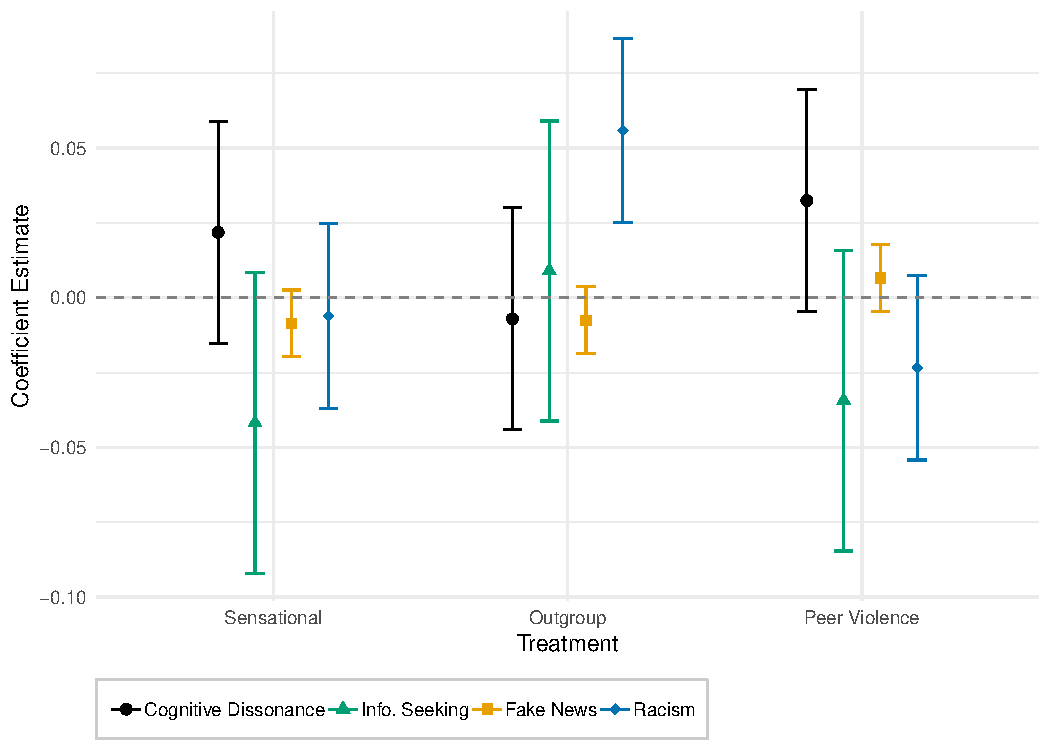
\includegraphics[width=.8\textwidth]{figures/additional_text_com.pdf}
\end{figure}

\newpage

\subsection{Coding Diagrams}

\begin{figure}[H]
  \centering
  \caption{Violence Coding Diagram}
  \vspace{1em}
  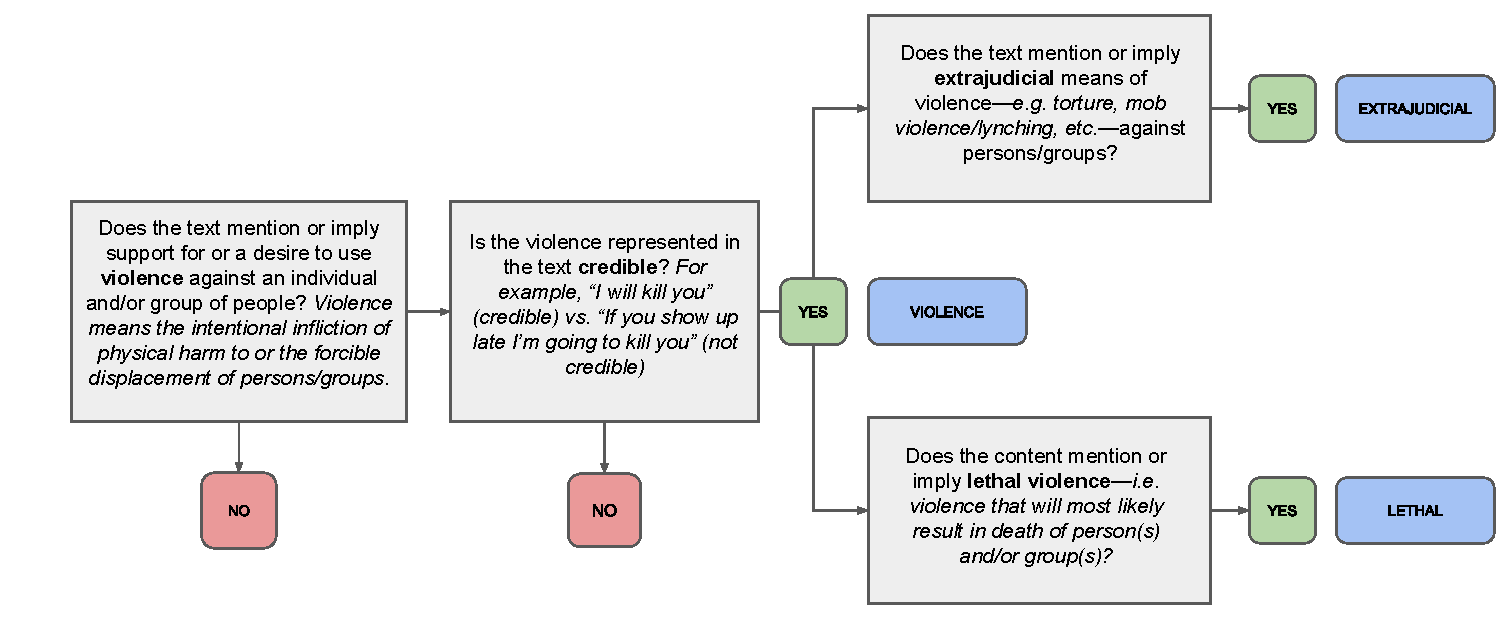
\includegraphics[width=.94\textwidth]{figures/Violence.pdf}\\
\end{figure}

%\begin{figure}[H]
%  \centering
%  \caption{Demonizing and Dehumanizing Coding Diagrams}
%  \vspace{1em}
%  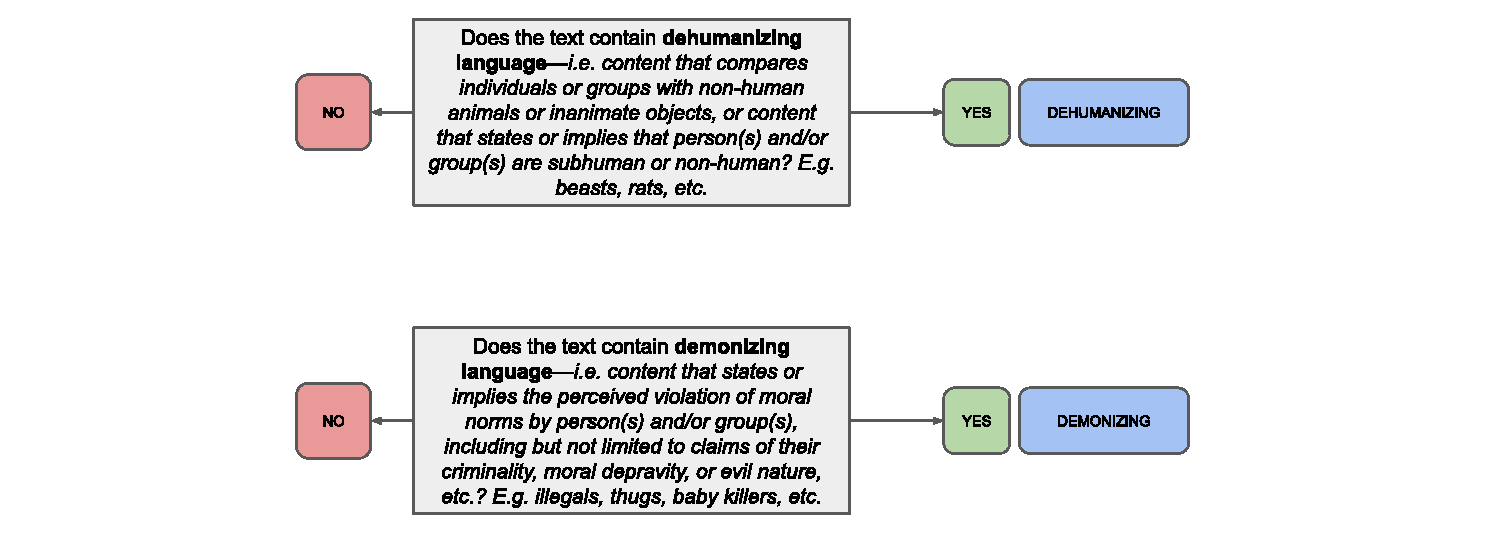
\includegraphics[width=.94\textwidth]{figures/DehumanizingDemonizing.pdf}\\
%\end{figure}

%\begin{figure}[H]
%  \centering
%  \caption{Group and Outgroup Coding Diagrams}
%  \vspace{1em}
%  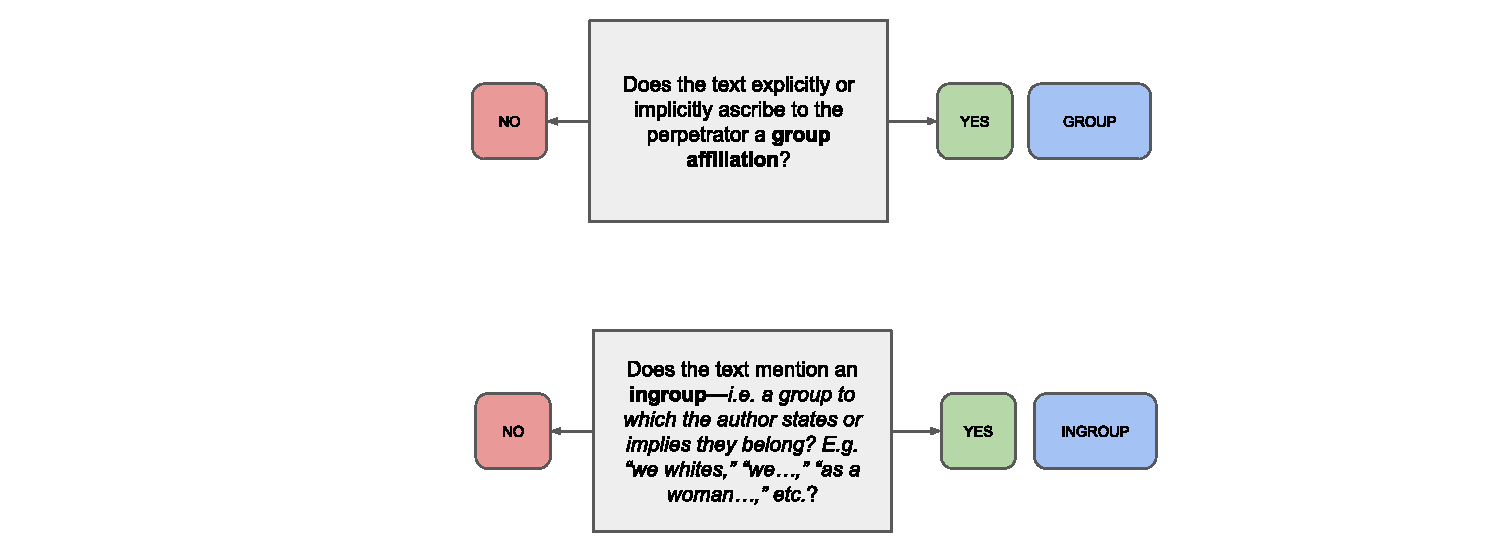
\includegraphics[width=.94\textwidth]{figures/GroupOutgroup.pdf}\\
%\end{figure}

%\begin{figure}[H]
%  \centering
%  \caption{Emotion Coding Diagrams}
%  \vspace{1em}
%  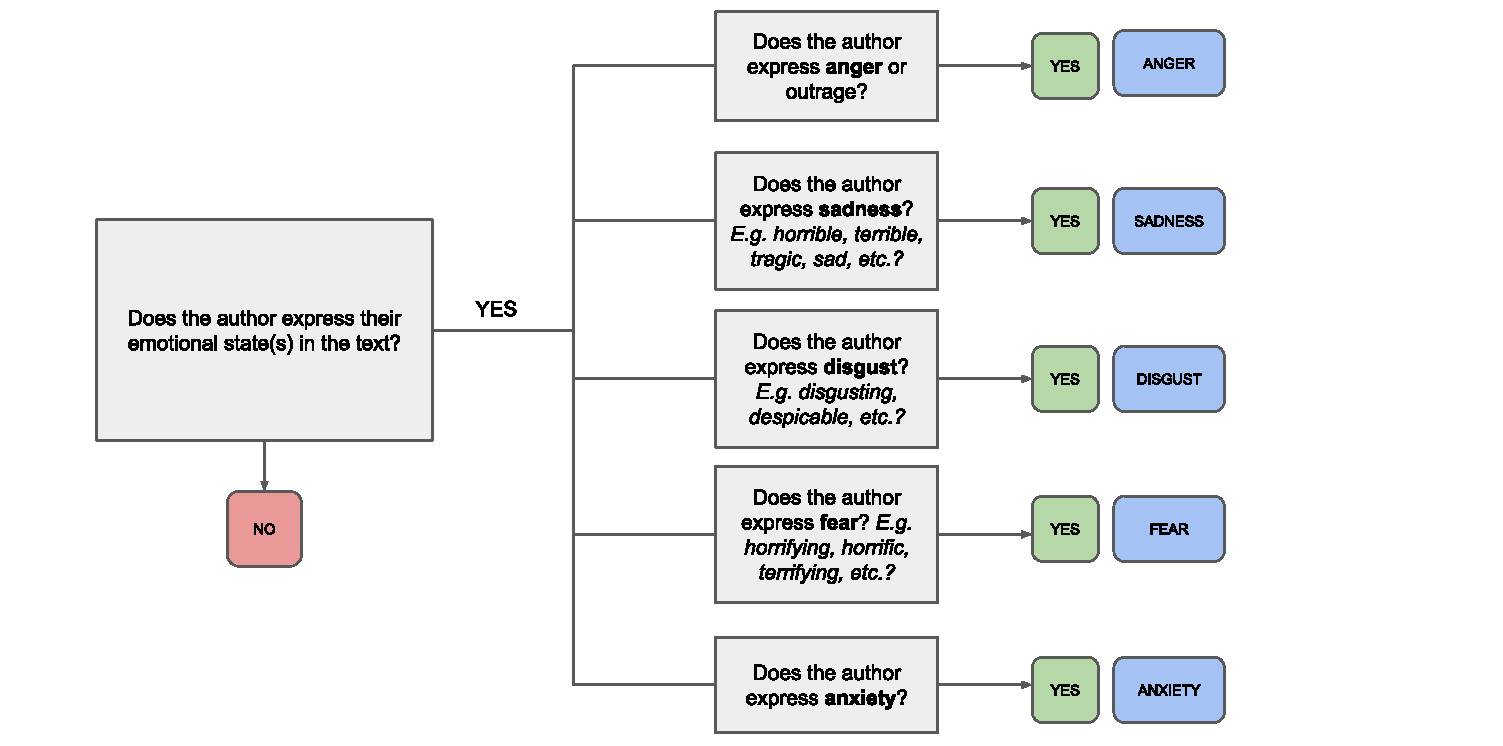
\includegraphics[width=.94\textwidth]{figures/Emotion.pdf}\\
%\end{figure}

\begin{figure}[H]
  \centering
  \caption{Racism and Social Desirability Coding Diagrams}
  \vspace{1em}
  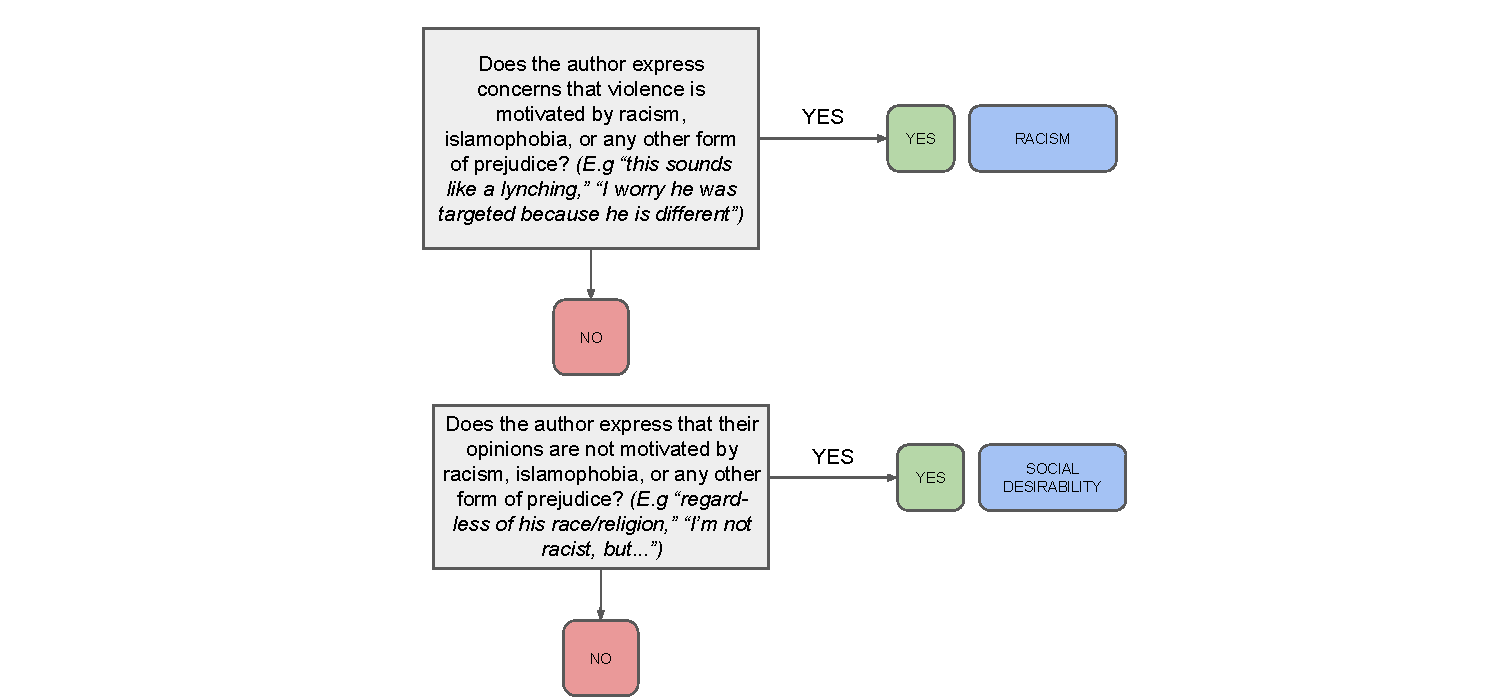
\includegraphics[width=.94\textwidth]{figures/RacismSocialDesirability.pdf}\\
\end{figure}

\begin{figure}[H]
  \centering
  \caption{Information-Seeking and Fake News Coding Diagrams}
  \vspace{1em}
  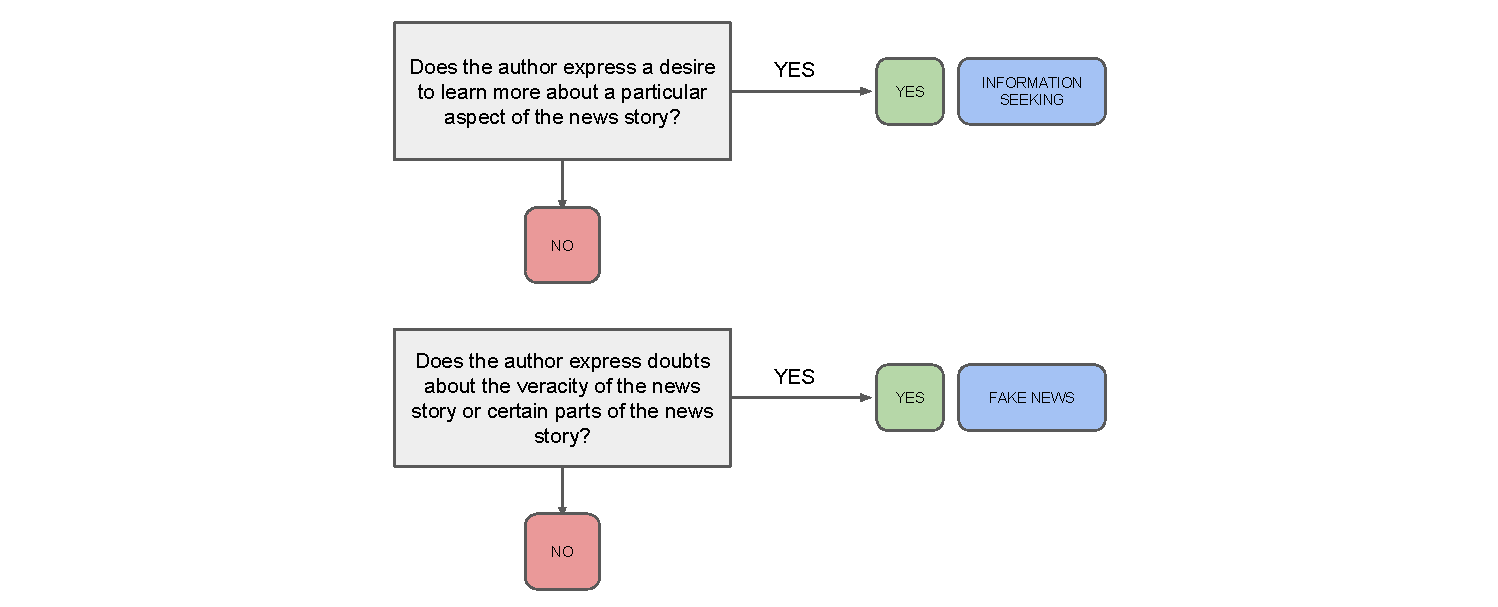
\includegraphics[width=.94\textwidth]{figures/InfoSeekingFakeNews.pdf}\\
\end{figure}

\begin{figure}[H]
  \centering
  \caption{Cognitive Dissonance Coding Diagrams}
  \vspace{1em}
  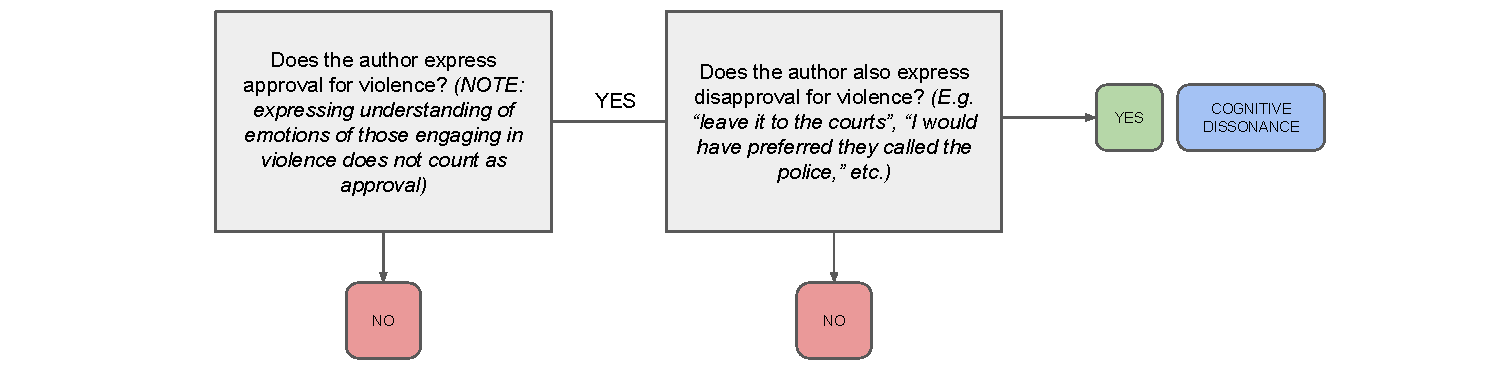
\includegraphics[width=.94\textwidth]{figures/CognitiveDissonance.pdf}\\
\end{figure}

\section{Intercoder Reliability}

% latex table generated in R 3.6.1 by xtable 1.8-4 package
% Wed Jul 24 16:53:47 2019
\begin{table}[ht]
\centering
\caption{Intercoder Reliability Measures} 
\begin{tabular}{lrr}
  \hline
Category & Kappa & F1 \\ 
  \hline
Cognitive Dissonance & 0.80 & 0.96 \\ 
  Fake News & 1.00 & 1.00 \\ 
  Info. Seeking & 0.71 & 0.93 \\ 
  Racism/Hate & 0.78 & 0.97 \\ 
  Social Desirability & 0.74 & 0.99 \\ 
  Violence & 0.81 & 0.90 \\ 
  Lethal Violence & 0.98 & 1.00 \\ 
  Extrajudicial Violence & 0.89 & 0.95 \\ 
 % Dehumanizing & 0.97 & 1.00 \\ 
 % Demonizing & 0.93 & 0.98 \\ 
 % Group & 0.95 & 0.99 \\ 
 % Ingroup & 0.93 & 0.98 \\ 
 % Anger & 0.94 & 0.99 \\ 
 % Disgust & 0.90 & 0.96 \\ 
 % Sadness & 0.89 & 0.93 \\ 
 % Fear & 0.91 & 0.99 \\ 
 % Anxiety & 0.88 & 0.99 \\ 
   \hline
\end{tabular}
\end{table}


\end{document}